
\documentclass[french]{article}
\usepackage[T1]{fontenc}
\usepackage[latin9]{inputenc}
\usepackage[paperwidth=18cm]{geometry}
\setcounter{secnumdepth}{0}
\setcounter{tocdepth}{5}
\usepackage{babel}
\makeatletter
\addto\extrasfrench{
   \providecommand{\og}{\leavevmode\flqq~}
   \providecommand{\fg}{\ifdim\lastskip>\z@\unskip\fi~\frqq}
}

\makeatother
\usepackage{float}
\usepackage[unicode=true,pdfusetitle,
 bookmarks=true,bookmarksnumbered=false,bookmarksopen=false,
 breaklinks=true,pdfborder={0 0 0},pdfborderstyle={},backref=false,colorlinks=false]
 {hyperref}

\makeatletter

\usepackage{algorithme}


\usepackage{pgf}
\usepackage{titlesec}
\usepackage{fancyhdr}
\pagestyle{fancy}
\fancyhead[C]{\sectiontitle}
\fancyhead[R]{
\includegraphics[scale=0.1]{logo.jpg}}
\lhead{Algorithmique : Projet Huffman}
\cfoot{\thepage}
\rfoot{\today}
\lfoot{Groupe 2.5}
\renewcommand{\headrulewidth}{0.4pt}

\setlength{\parindent}{0cm}
\setlength{\parskip}{1ex plus 0.5ex minus 0.2ex}
\newcommand{\hsp}{\hspace{20pt}}
\newcommand{\HRule}{\rule{\linewidth}{0.5mm}}
\usepackage{minted}
\usepackage{caption}
\usepackage{color}
\definecolor{bg}{rgb}{0.95,0.95,0.95}

\newmintedfile[cc]{c}{linenos=true,mathescape,bgcolor=bg}


\usepackage{graphicx}

\makeatother

\begin{document}
 
\begin{titlepage}
	\begin{sffamily}
	\begin{center}
\textsc{\LARGE INSA DE ROUEN}\\[1cm]

\includegraphics[scale=0.35]{page_de_garde_1.png}\\[1cm]

\textsc{\Large Rapport de projet d'algorithmique}\\[1cm]

\HRule \\[0.4cm]
{\huge \bfseries Compresseur d'Huffman\\[0.4cm]}

\HRule \\[1cm]
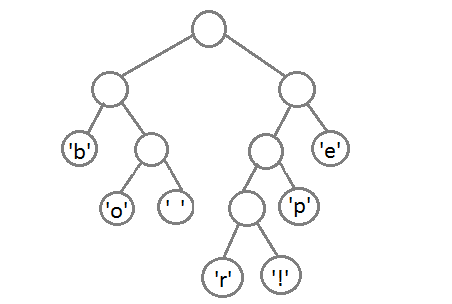
\includegraphics[scale=0.6]{page_de_garde_2.png}
\\[1cm]

\begin{minipage}{0.4\linewidth}
\begin{flushleft} \large
Tshora Leonard\\
Tharmarajah Assvin\\
Talout Salim\\
Tiphagne Thomas\\
Russias Sylvie\\
\end{flushleft}
\end{minipage}
\hfill
\begin{minipage}{0.4\linewidth}
\begin{flushright} \large
\emph{Professeur :} M. Delestre
\end{flushright}
\end{minipage}
\vfill
{\large Ann�e 2016 - 2017}


\end{center}
\end{sffamily}
\end{titlepage}

\newpage

\tableofcontents{}

\newpage

\part{Introduction}

Dans le cadre du cours "Algorithmique avanc�e et programmation C", nous devions concevoir un compresseur utilisant l'algorithme de Huffman. Cette m�thode consiste en l'utilisation d'un code � longueur variable pour repr�senter un symbole du fichier source. Le code est d�termin� � partir de la fr�quence d'apparition des symboles de source, un code court �tant associ� aux symboles de source les plus fr�quents. Ainsi, un symbole fr�quent � un code plus court qu'un caract�re n'apparaissant qu'un nombre limit� de fois.
Pour concevoir cet algorithme, nous avons utilis� un arbre binaire dont les feuilles sont des �l�ments du fichier source, ainsi le code correspondant � chaque caract�re est le chemin permettant d?atteindre ces �l�ments.

Notre groupe �tant form� de 5 personnes (Assvin, Leonard, Salim, Thomas et Sylvie), nous avons d� mettre en pratique nos comp�tences et connaissances afin de mener � bien ce projet d'une dur�e de 10 semaines. Dans ce rapport, nous expliciterons donc les �tapes principales du projet, en suivant un cycle en V, en allant de l'analyse jusqu'aux tests.


\newpage

\part{Analyses}

\section{Pr�sentation des TAD :}

\subsection{Octet :}

\begin{tad}
	\tadNom{Octet}
	\tadDependances{\booleen, \naturel, Bit}
	\begin{tadOperations}{Octet}
		\tadOperation{creerOctet}{}{\tadUnParam{Octet}}
		\tadOperationAvecPreconditions{obteniriemeBit}{\tadDeuxParams{Octet}{\naturel}}{\tadUnParam{Bit}}				
		\tadOperation{fixeriemeBit}{\tadTroisParams{Octet}{Bit}{\naturel}}{\tadUnParam{Octet}}
		\tadOperation{octetsEgaux}{\tadDeuxParams{Octet}{Octet}}{\tadUnParam{\booleen}}
		\tadOperationAvecPreconditions{decimalEnOctet}{\tadUnParam{Entier}}{\tadUnParam{Octet}}
		\tadOperation{octetEnDecimal}{\tadUnParam{Octet}}{\tadUnParam{Entier}}
		\tadOperation{copierOctet}{\tadUnParam{Octet}}{\tadUnParam{Octet}}

	\end{tadOperations}

	\begin{tadPreconditions}{}
		\tadPrecondition{obteniriemeBit(i)}{1<=i<=8}
		\tadPrecondition{decimalEnOctet(dec)}{0<=dec<=255}

	\end{tadPreconditions}

\end{tad}


\subsection{Arbre de Huffman :}

\begin{tad}
	\tadNom{ArbreDeHuffman}
	\tadParametres{Element}
	\tadDependances{Booleen}
	\begin{tadOperations}{Arbre de Huffman}
		\tadOperation{creerArbreDeHuffmanVide}{}{\tadUnParam{ArbreDeHuffman}}
		\tadOperation{creerArbreDeHuffman}{\tadDeuxParams{Octet}{Naturel}}{\tadUnParam{ArbreDeHuffman}}
		\tadOperation{estUneFeuille}{\tadUnParam{ArbreDeHuffman}}{\tadUnParam{Booleen}}
		\tadOperation{estVide}{\tadUnParam{ArbreDeHuffman}}{\tadUnParam{\booleen}}
		\tadOperationAvecPreconditions{obtenirPere}{\tadUnParam{ArbreDeHuffman}}{\tadUnParam{Element}}
		\tadOperationAvecPreconditions{obtenirFilsGauche}{\tadUnParam{ArbreDeHuffman}}{\tadUnParam{ArbreDeHuffman}}
		\tadOperationAvecPreconditions{obtenirFilsDroit}{\tadUnParam{ArbreDeHuffman}}{\tadUnParam{ArbreDeHuffman}}
		\tadOperation{fusionnerArbreDeHuffman}{\tadDeuxParams{ArbreDeHuffman}{ArbreDeHuffman}}{\tadUnParam{ArbreDeHuffman}}
		\tadOperation{comparerArbreDeHuffman}{\tadDeuxParams{ArbreDeHuffman}{ArbreDeHuffman}}{\tadUnParam{Booleen}}
	\end{tadOperations}
	\begin{tadSemantiques}{}
		\tadSemantique{obtenirPere}{Retourne l'�lement pr�sent dans l'arbre (ne remonte pas d'un cran!)}
		\end{tadSemantiques}
	\begin{tadAxiomes}
		\tadAxiome{estUneFeuille(CreerArbreHuffman())=Vrai}
	\end{tadAxiomes}
	
	\begin{tadPreconditions}{}
		\tadPrecondition{obtenirFilsGauche(a)}{non(estUneFeuille(a))}
		\tadPrecondition{obtenirFilsDroit(a)}{non(estUneFeuille(a)))}
		\tadPrecondition{obtenirRacine(a)}{non(estVide(a))}
	\end{tadPreconditions}
\end{tad}


\subsection{Statistiques :}


\signaturefonction{creerVide}{}{Statistiques}
\signaturefonction{estVide}{Statistiques}{Booleen}
\signaturefonction{estPresentItem}{stats : Statistiques, oct : octet}{Booleen}
\signaturefonction{taille}{stats : Statistiques}{Naturel}
\signaturefonction{nombreOccurencesItem}{stats : Statistiques,item : Item}{Naturel}
\signatureprocedure{fixerOccurencesItem}{E/S stats : Statistiques, E item : Item, nombre : Naturel}
\signatureprocedure{supprimerItem}{E/S stats : Statistiques, E position : Naturel}
\signatureprocedure{ajouterItem}{E/S stats : Statistiques, E item : Item}
\signaturefonction{obtenirItem}{E/S stats : Statistiques, E position : Naturel}{oct : Octet,ponderation : Naturel}


\subsection{File de priorit�s :}

\begin{tad}
	\tadNom{FileDePriorit�}
	\tadParametres{Item}
	\tadDependances{\booleen,\naturel}
	\begin{tadOperations}{FileDePriorit�}
		\tadOperation{creerVide}{}{\tadUnParam{FileDePriorit�}}
		\tadOperation{estVide}{\tadUnParam{FileDePriorit�}}{\tadUnParam{\booleen}}
		\tadOperationAvecPreconditions{defiler} {\tadUnParam{FileDePriorit�}} {\tadUnParam{FileDePriorit�}}
		\tadOperation{insererItem}{\tadTroixParams{FileDePriorite}{Item}{\booleen}} {\tadUnParam{FileDePriorite}}
		\tadOperationAvecPreconditions{obtenirTete}{\tadUnParam{FileDePriorite}} {\tadUnParam{Item}}
		\tadOperation{longueur}{\tadUnParam{FileDePriorite}} {\tadUnParam{Naturel}}
	\end{tadOperations}
	\begin{tadSemantiques}{Statistiques}
		\tadSemantique{defiler}{Supprime l'Item en t�te de liste (le premier � sortir).}
		\tadSemantique{insererItem}{Ins�re l'Item au bon endroit dans la liste. Il faut donc �tre capable de comparer deux Items.}
		\tadSemantique{obtenirTete}{Donne l'Item en t�te de liste (premier � sortir)}
	\end{tadSemantiques}
	\begin{tadPreconditions}{}
		\tadPrecondition{defiler(f)} {non(estVide(f))}
		\tadPrecondition{obtenirTete(f)} {non(estVide(f))}
	\end{tadPreconditions}
\end{tad}


\subsection{Code binaire :}

 \begin{tad}
  \tadNom{Code Binaire}
  \tadDependances{Bit,Naturel}
  \begin{tadOperations}{Code Binaire}
   \tadOperation{CreerCodeBinaireVide}{}{\tadUnParam{Code Binaire}}
   \tadOperation{estVide}{\tadUnParam{Code Binaire}}{\tadUnParam{Booleen}}
   \tadOperationAvecPreconditions{obtenirBit}{\tadUnParam{Code Binaire}}{\tadUnParam{Bit}}
   \tadOperationAvecPreconditions{obtenirIemeBitCodeBinaire}{\tadDeuxParams{Code Binaire}{Naturel Non Nul}}{\tadUnParam{Bit}}
   \tadOperation{obtenirLongueur}{\tadUnParam{Code Binaire}}{\tadUnParam{Naturel Non Nul}}
   \tadOperation{obtenirCodeBinaireSuivant}{\tadUnParam{Code Binaire}}{\tadUnParam{Code Binaire}}
   \tadOperationAvecPreconditions{fixerCodeBinaireSuivant}{\tadUnParam{Code Binaire}}{\tadUnParam{Code Binaire}}
   \tadOperationAvecPreconditions{supprimerTete}{\tadUnParam{Code Binaire}}{\tadUnParam{Code Binaire}}
   \tadOperationAvecPreconditions{supprimerBit}{\tadDeuxParams{Code Binaire}{Naturel Non Nul}}{\tadUnParam{Code Binaire}}
   \tadOperation{supprimer}{\tadUnParam{Code Binaire}}{}
   \tadOperation{ajouterEnTete}{\tadDeuxParams{Code Binaire}{Bit}}{\tadUnParam{Code Binaire}}
   \tadOperationAvecPreconditions{ajouterBit}{\tadTroisParams{Code Binaire}{Bit}{Naturel}}{\tadUnParam{Code Binaire}}
   \tadOperation{ajouterAlaFin}{\tadDeuxParams{Code Binaire}{Bit}}{\tadUnParam{Code Binaire}}
   \tadOperation{sontEgaux}{\tadDeuxParams{Code Binaire}{Code Binaire}}{\tadUnParam{Booleen}}
   \tadOperation{concatener}{\tadDeuxParams{Code Binaire}{Code Binaire}}{\tadUnParam{Code Binaire}}
   \tadOperation{copierCodeBinaire}{\tadUnParam{Code Binaire}}{\tadUnParam{Code Binaire}}
   \tadOperation{convertirCodeBinaireEnBaseDix}{\tadUnParam{Code Binaire}}{\tadUnParam{Entier}}
  \end{tadOperations}
  \begin{tadPreconditions}{}
    	\tadPrecondition{obtenirBit(Code)}{non(estVide(Code))}
  	\tadPrecondition{obtenirIemeBitCodeBinaire(Code,i)}{i>0, i<obtenirLongueur(Code)}
  	\tadPrecondition{fixerCodeBinaireSuivant(C1,C2)}{non(estVide(C1))}
  	\tadPrecondition{supprimerTete(Code)}{non(estVide(Code))}
  	\tadPrecondition{supprimerBit(Code, i)}{i>0, i<obtenirLongueur(Code)}
  	\tadPrecondition{ajouterBit(Code, i, b)}{i>0, i<obtenirLongueur(Code)}


  \end{tadPreconditions}
 \end{tad}



\subsection{Table de codage :}

\signaturefonction {tableDeCodageVide}{}{\TableDeCodage}

\procedure {ajouterElement} {\paramEntree{element:\Octet}} {\paramEntreeSortie{table:\TableDeCodage}}

précondition(s) non(estPresent(table, element))

\procedure {fixerCodeElement} {\paramEntree{element:\Octet, mon_code_binaire:\CodeBinaire}} {\paramEntreeSortie{table:\TableDeCodage}} 

précondition(s) estPresent(table, element)

\procedure {supprimerElement} {\paramEntree{element:\Octet}} {\paramEntreeSortie{table:TableDeCodage}}

précondition(s) estPresent(table, element)

\signaturefonction {estPresentElement}{table:\TableDeCodage, element:\Octet}{\Booléen}

\signaturefonction {estPresentCodeBinaire}{table:\TableDeCodage, mon_code_binaire:\CodeBinaire}{\Booléen}

\signaturefonction {obtenirCode}{table:\TableDeCodage, element:\Octet}{\CodeBinaire}

précondition(s) estPresentElement(table,element)

\signaturefonction {obtenirElement}{table:\TableDeCodage, mon_code_binaire:\CodeBinaire}{\Octet}

précondition(s) estPresentCodeBinaire(table,mon_code_binaire)


\newpage

\section{Pr�sentation de l'analyse descendante :}
\begin{center}
\includegraphics[angle=90,scale=0.35]{\string"analyses/partie droite\string".pdf}
\par\end{center}

\begin{center}
\includegraphics[angle=90,scale=0.07]{\string"analyses/partie gauche\string".pdf}
\par\end{center} 


\newpage

\part{Conception pr�liminaire}

\section{Conception pr�liminaire des TAD :}

\subsection{Octet :}

 
\begin{algorithme}

\signaturefonction
{creerOctet}
{}
{Octet}


\signatureProcedure
{fixeriemeBit}
{\paramEntreeSortie{o : Octet} ; \paramEntree{i : \naturel, b : Bit}}

\signatureFonction
{obteniriemeBit}
{o : Octet, indice : Naturel}
{Bit}


\signaturefonction
{octetsEgaux}
{o1, o2 : Octet}
{\booleen}

\end{algorithme}

\subsection{Code Binaire :}

 \begin{algorithme}

\signaturefonction 
{fichierBinaire}
{c : Chaine}
{fichierBinaire}

\signaturefonction
{ouvrir}
{chaine, FBmode}
{fichierBinaire}

\signatureprocedure
{fermer}
{\paramEntreeSortie{f : FichierBinaire}}

\signaturefonction
{estOuvert}
{f: FichierBinaire}
{\booleen}

\signaturefonction
{mode}
{f: FichierBinaire}
{Mode}

\signaturefonction
{finFichier}
{f: FichierBinaire}
{\booleen}

\signatureprocedure
{ecrireOctet}
{\paramEntreeSortie{f : FichierBinaire} ; \paramEntree{o : Octet}}

\signatureprocedure
{lireOctet}
{\paramEntreeSortie{f : FichierBinaire} ; \paramSortie{o : Octet}}

\signatureprocedure
{ecrireNaturel}
{\paramEntreeSortie{f : FichierBinaire} ; \paramEntree{a : Naturel}}

\signatureprocedure
{lireNaturel}
{\paramEntreeSortie{f : FichierBinaire} ; \paramSortie{a :  Naturel}}

\signatureprocedure
{ecrireCaractere}
{\paramEntreeSortie{f : FichierBinaire} ; \paramEntree{c : \caractere}}

\signatureprocedure
{lireCaractere}
{\paramEntreeSortie{f : FichierBinaire} ; \paramSortie{c : \caractere}}

\signatureprocedure
{deplacerCurseurPourTrouverTaille}
{\paramEntreeSortie{f : FichierBinaire}}

\end{algorithme}


\subsection{Table de Codage :}

 
\begin{algorithme}

\signaturefonction 
{tableDeCodageVide}
{}
{TableDeCodage}

\signatureprocedure
{fixerCodeElement}
{\paramEntreeSortie{t : TableDeCodage} ; \paramEntree{o : Octet, c : CodeBinaire}}


\signatureFonctionAvecPreconditions
{obtenirCodeBinaire}
{t : TableDeCodage, o : Octet}
{CodeBinaire}
{octetPresent(o)}

\end{algorithme}

\subsection{Statistiques :}

 
\begin{algorithme}


\signaturefonction
{creerVide}
{}
{Statistiques}

\signaturefonction
{estVide}
{stats : Statistiques}
{\booleen}

\signatureprocedure
{fixerOccurenceItem}
{\paramEntreeSortie{stats : Statistiques} ; \paramEntree{o : Octet}}

\signatureProcedureAvecPreconditions
{ajouterItem}
{\paramEntreeSortie{stats : Statistiques} ; \paramEntree{o : Octet , nb : \naturel}}
{non estPresent(stats,o)}

\signatureProcedure
{ajouterItemALaFin}
{\paramEntreeSortie{stats : Statistiques} ; \paramEntree{o : Octet , nb : \naturel}}


\signatureFonctionAvecPreconditions
{nombreOccurencesItem}
{stats : Statistiques, o : Octet}
{\naturel}
{estPresent(stats,o)}

\signaturefonction
{estPresent}
{stats : Statistiques, o : octet}
{\booleen}

\signatureFonction
{obtenirOctet}
{donnee : donneeNoeud}
{Octet}

\signatureProcedure
{obtenirStatSuivante}
{\paramEntreeSortie{s : Statistiques}

\end{algorithme}


\subsection{Arbre De Huffman :}

 
\begin{algorithme}

\signaturefonction 
{ADH\_creerArbreDeHuffmanVide}
{}
{ADH\_arbreDeHuffman}

\signaturefonction 
{ADH\_creerArbreDeHuffman}
{octetAAjouter : octet, ponderation : \naturel}
{ADH\_arbreDeHuffman}

\signaturefonction 
{ADH\_estUneFeuille}
{arbre : ADH\_arbreDeHuffman}
{\booleen}

\signaturefonction 
{ADH\_obtenirPere}
{arbre : ADH\_arbreDeHuffman}
{ADH\_valeurRacine}

\signaturefonction 
{ADH\_obtenirFilsD/G}
{arbre : ADH\_arbreDeHuffman}
{ADH\_arbreDeHuffman}

\signaturefonction 
{ADH\_estVide}
{arbre : ADH\_arbreDeHuffman}
{\booleen}

\signaturefonction 
{ADH\_creerRacine}
{octetAAjoute: Octet, ponderation : Entier}
{ADH\_Racine}

\signaturefonction 
{ADH\_fusionnerArbreDeHuffman}
{arbre1, arbre2 : ADH\_arbreDeHuffman}
{ADH\_arbreDeHuffman}

\signaturefonction 
{ADH\_comparerArbreDeHuffman}
{arbre1, arbre2 : ADH\_arbreDeHuffman}
{\booleen}

\signatureProcedure
{FDP\_supprimerRacine}
{\paramEntreeSortie{arbreDeHuffman}}

\signatureProcedure
{FDP\_supprimer}
{\paramEntreeSortie{arbreDeHuffman}}
\end{algorithme}


\subsection{File De Priorite :}


\begin{algorithme}

 \signaturefonction
{FDP\_creerVide}
{}
{fileDePriorite}

\signaturefonction
{FDP\_estVide}
{file : fileDePriorite}
{\booleen}

 \signaturefonction
{obtenirTete}
{file : fileDePriorite}
{ADH\_arbreDeHuffman}

\signaturefonction
{FDP\_longueur}
{file : fileDePriorite}
{\naturel}

\signatureProcedure
{FDP\_defiler}
{\paramEntreeSortie{fileDePriorite}}


\signatureProcedure
{FDP\_supprimer}
{\paramEntreeSortie{fileDePriorite}}


\signatureProcedure
{FDP\_insererItem}
{\paramEntree{arbreeDeHuffman, param : \booleen}, \paramEntreeSortie{fileDePriorite}}


\end{algorithme}


\subsection{Fichier Binaire :}

 \begin{algorithme}

\signaturefonction 
{fichierBinaire}
{c : Chaine}
{fichierBinaire}

\signaturefonction
{ouvrir}
{chaine, FBmode}
{fichierBinaire}

\signatureprocedure
{fermer}
{\paramEntreeSortie{f : FichierBinaire}}

\signaturefonction
{estOuvert}
{f: FichierBinaire}
{\booleen}

\signaturefonction
{mode}
{f: FichierBinaire}
{Mode}

\signaturefonction
{finFichier}
{f: FichierBinaire}
{\booleen}

\signatureprocedure
{ecrireOctet}
{\paramEntreeSortie{f : FichierBinaire} ; \paramEntree{o : Octet}}

\signatureprocedure
{lireOctet}
{\paramEntreeSortie{f : FichierBinaire} ; \paramSortie{o : Octet}}

\signatureprocedure
{ecrireNaturel}
{\paramEntreeSortie{f : FichierBinaire} ; \paramEntree{a : Naturel}}

\signatureprocedure
{lireNaturel}
{\paramEntreeSortie{f : FichierBinaire} ; \paramSortie{a :  Naturel}}

\signatureprocedure
{ecrireCaractere}
{\paramEntreeSortie{f : FichierBinaire} ; \paramEntree{c : \caractere}}

\signatureprocedure
{lireCaractere}
{\paramEntreeSortie{f : FichierBinaire} ; \paramSortie{c : \caractere}}

\signatureprocedure
{deplacerCurseurPourTrouverTaille}
{\paramEntreeSortie{f : FichierBinaire}}

\end{algorithme}


\section{Conception pr�liminaire du programme :}

\subsection{ecrireCodeBinaire :}


\begin{algorithme}
	\signatureprocedure{ecrireCodeBinaire}{\paramEntree{table : TableDeCodage, nb : \entier }\paramSortie{fichierFinal : FichierBinaire}}
	

\end{algorithme}

		


\subsection{ecrireEnTete :}


\begin{algorithme}

	\signatureprocedure{ecrireEnTete}{\paramEntree{statistique : Statistiques }\paramEntreeSortie{fichierCompresse : FichierBinaire}}
	\signatureprocedure{ecrireCodeIdentification}{\paramEntreeSortie{fichierCompresse : FichierBinaire}}
	\signatureprocedure{ecrireTaille}{\paramEntree{taille : \entier }\paramEntreeSortie{fichierCompresse : FichierBinaire}}
	\signatureprocedure{ecrireStatistiques}{\paramEntree{statistique : statistiques }\paramEntreeSortie{fichierCompresse : FichierBinaire}}


\end{algorithme}

		


\subsection{decoder :}

\begin{minted}[breaklines=true,linenos=true,mathescape,bgcolor=bg]{c}

#include "decoder.h"




void decoder(ADH_arbreDeHuffman arbre,FichierBinaire source, FichierBinaire* dest,int longueur,CLC_FonctionCopier copierBit,CLC_FonctionLiberer libererBit){

	unsigned long long bit_restants=longueur,i;
	octet o;
	CodeBinaire cTemp,code=CB_creerCodeBinaireVide();

	while (!(FB_finFichier(source)) && FB_lireOctet(source,&o) && (bit_restants>0)) {
		
	
		cTemp=octet_en_CB(o,copierBit);		
		CB_concatener(&code,cTemp);
		while ((CB_obtenirLongueur(code)>=NB_MAX_BITS) && (bit_restants>0)) {
			traiterCodeBinaire(&code, &o, &bit_restants, arbre, libererBit);
			FB_ecrireOctet(dest,o);
		}
	}

}


void traiterCodeBinaire(CodeBinaire* code,octet* oct,unsigned long long* nb,ADH_arbreDeHuffman arbre,CLC_FonctionLiberer libererBit)
{
	unsigned int i;
	int l=CB_obtenirLongueur(*code);
	ADH_arbreDeHuffman atemp=arbre;

	if (l>(*nb))
	{
		for (i=l;i>*nb;i--)
		{
			CB_supprimerBit(code,i,libererBit);
		}
		assert(*nb==CB_obtenirLongueur(*code));
	}
	while (!(ADH_estUneFeuille(atemp)))
	{
		*nb=*nb-1;
		if (bit_egaux(CB_obtenirBit(*code),b0))
		{
			atemp=ADH_obtenirFilsGauche(atemp);
		}
		else atemp=ADH_obtenirFilsDroit(atemp);
		CB_supprimerTete(code,libererBit);
	}
	copierOctet(ADH_obtenirPere(atemp).valeurOctet,oct);

}

CodeBinaire octet_en_CB(octet oct,CLC_FonctionCopier copierBit)
{
	int i=0;
	CodeBinaire res=CB_creerCodeBinaireVide();
	for (i=0;i<8;i++)
		{
			CB_ajouterAlaFin(&res, obteniriemeBit(oct, i), copierBit);
		}
	return res;
}

\end{minted}
 


\subsection{genererArbre :}


\begin{algorithme}
\small
	\signaturefonction{genererArbre}{file : File de Priorite, copierArbre : Fonction Copier}{arbre : Arbre de Huffman}
	\signatureprocedure{genererArbreRecursivement}{\paramEntree{file : fileDePriorite, copierArbre : FonctionCopier, }}
	


\end{algorithme}

		

\subsection{genererFileDePriorite :}

\begin{algorithme}

\signaturefonction{genererFileDePriorite}{stats : Statistiques, param : \booleen, }{fileDePriorite}
\end{algorithme}


\subsection{genererTDCAPartirDeADH :}

\begin{algorithme}
\signaturefonction{genererTableDeCodageAPArtirDeArbre}{arbre : ArbreDeHuffman}{table : TableDeCodage}
\signatureprocedure{chercherFeuilleRecur}{E/S  : arbre : ArbreDeHuffman, code : CodeBinaire, table : TableDeCodage}
\end{algorithme}


\subsection{Autres :}

\begin{algorithme}

\signaturefonction{compresser}{fichierACompresser : fichierBinaire}{fichierBinaire}
\signaturefonction{estCompressible}{fichier : fichierBinaire}{Booleen}
\signaturefonction{estCompresse}{fichier : fichierBinaire}{Booleen}
\signaturefonction{genererTableDeCodageAPartirDeStats}{stats : statistiques}{tableDeCodage}
\signaturefonction{decompresser}{fichierADecompresser : fichierBinaire}{fichierBinaire}

\end{algorithme}
 


\newpage

\part{Conception d�taill�e}

 \section{Conception d�taill�e des TAD :}

\subsection{Octet :}


\begin{algorithme}
  \begin{enregistrement}{Octet}
    \champEnregistrement{lesBits}{\tableauUneDimension{1..8}{de }{Bit}}
  \end{enregistrement}

  \fonction{creerOctet}
{}
{Octet}
{resultat : Octet, i : NaturelNonNul}
{
   \pour{i}{1}{NBMAXBITS}{}
   {
       \affecter{resultat.lesBits[i]}{b0}
   }
   \retourner{resultat}
}

\fonctionAvecPreconditions
{OCT.obteniriemeBit}
{UnOctet : Octet, i : \naturel}
{Bit}
{i<=NBMAXBITS}
{}
  {
    \retourner{UnOctet.LesBits[i]}
  }

    \fonction{octetEgaux}
{Octet1, Octet2 : Octet}
{\booleen}
{resultat : \booleen, i : NaturelNonNul}
{
  \affecter{resultat}{Vrai}
   \pour{i}{1}{NBMAXBITS}{}
   {
      \sialors{Octet1.LesBits[i]!=Octet2.LesBits[i]}
      {

       \affecter{resultat}{Faux}
   }}
   \retourner{resultat}
}

\fonction
{octetEnDecimal}
{oct : octet}
{\naturel}
{i, res : \naturel}
{
\affecter{res}{0}
\pour{i}{7}{0}{}{
\affecter{res}{res+bit\_en\_int(oct.lesBits[NB\_MAX\_BITS-i-1])*(int)pow((double)2,(double)i)}
}
\retourner{res}
}

\fonctionAvecPreconditions
{decimalEnOctet}
{dec : \naturel}
{octet}
{dec $\geq$ 0 ET dec $\leq$ 255}
{i, temp, coeff : \naturel, res : octet}
{
\affecter{temp}{dec}
\pour{i}{NB\_MAX\_BITS-1}{0}{}
{
\affecter{coeff}{pow(2,i)}
\instruction{fixeriemeBit(res,NB\_MAX\_BITS-i-1,int\_en\_bit(temp/coeff))}
\affecter{temp}{temp-coeff*(temp/coeff)}
}
\retourner{res}
}

\end{algorithme}



\subsection{Code Binaire :}

 \begin{tad}
  \tadNom{Code Binaire}
  \tadDependances{Bit,Naturel}
  \begin{tadOperations}{Code Binaire}
   \tadOperation{CreerCodeBinaireVide}{}{\tadUnParam{Code Binaire}}
   \tadOperation{estVide}{\tadUnParam{Code Binaire}}{\tadUnParam{Booleen}}
   \tadOperationAvecPreconditions{obtenirBit}{\tadUnParam{Code Binaire}}{\tadUnParam{Bit}}
   \tadOperationAvecPreconditions{obtenirIemeBitCodeBinaire}{\tadDeuxParams{Code Binaire}{Naturel Non Nul}}{\tadUnParam{Bit}}
   \tadOperation{obtenirLongueur}{\tadUnParam{Code Binaire}}{\tadUnParam{Naturel Non Nul}}
   \tadOperation{obtenirCodeBinaireSuivant}{\tadUnParam{Code Binaire}}{\tadUnParam{Code Binaire}}
   \tadOperationAvecPreconditions{fixerCodeBinaireSuivant}{\tadUnParam{Code Binaire}}{\tadUnParam{Code Binaire}}
   \tadOperationAvecPreconditions{supprimerTete}{\tadUnParam{Code Binaire}}{\tadUnParam{Code Binaire}}
   \tadOperationAvecPreconditions{supprimerBit}{\tadDeuxParams{Code Binaire}{Naturel Non Nul}}{\tadUnParam{Code Binaire}}
   \tadOperation{supprimer}{\tadUnParam{Code Binaire}}{}
   \tadOperation{ajouterEnTete}{\tadDeuxParams{Code Binaire}{Bit}}{\tadUnParam{Code Binaire}}
   \tadOperationAvecPreconditions{ajouterBit}{\tadTroisParams{Code Binaire}{Bit}{Naturel}}{\tadUnParam{Code Binaire}}
   \tadOperation{ajouterAlaFin}{\tadDeuxParams{Code Binaire}{Bit}}{\tadUnParam{Code Binaire}}
   \tadOperation{sontEgaux}{\tadDeuxParams{Code Binaire}{Code Binaire}}{\tadUnParam{Booleen}}
   \tadOperation{concatener}{\tadDeuxParams{Code Binaire}{Code Binaire}}{\tadUnParam{Code Binaire}}
   \tadOperation{copierCodeBinaire}{\tadUnParam{Code Binaire}}{\tadUnParam{Code Binaire}}
   \tadOperation{convertirCodeBinaireEnBaseDix}{\tadUnParam{Code Binaire}}{\tadUnParam{Entier}}
  \end{tadOperations}
  \begin{tadPreconditions}{}
    	\tadPrecondition{obtenirBit(Code)}{non(estVide(Code))}
  	\tadPrecondition{obtenirIemeBitCodeBinaire(Code,i)}{i>0, i<obtenirLongueur(Code)}
  	\tadPrecondition{fixerCodeBinaireSuivant(C1,C2)}{non(estVide(C1))}
  	\tadPrecondition{supprimerTete(Code)}{non(estVide(Code))}
  	\tadPrecondition{supprimerBit(Code, i)}{i>0, i<obtenirLongueur(Code)}
  	\tadPrecondition{ajouterBit(Code, i, b)}{i>0, i<obtenirLongueur(Code)}


  \end{tadPreconditions}
 \end{tad}



\subsection{Table de Codage :}

\signaturefonction {tableDeCodageVide}{}{\TableDeCodage}

\procedure {ajouterElement} {\paramEntree{element:\Octet}} {\paramEntreeSortie{table:\TableDeCodage}}

précondition(s) non(estPresent(table, element))

\procedure {fixerCodeElement} {\paramEntree{element:\Octet, mon_code_binaire:\CodeBinaire}} {\paramEntreeSortie{table:\TableDeCodage}} 

précondition(s) estPresent(table, element)

\procedure {supprimerElement} {\paramEntree{element:\Octet}} {\paramEntreeSortie{table:TableDeCodage}}

précondition(s) estPresent(table, element)

\signaturefonction {estPresentElement}{table:\TableDeCodage, element:\Octet}{\Booléen}

\signaturefonction {estPresentCodeBinaire}{table:\TableDeCodage, mon_code_binaire:\CodeBinaire}{\Booléen}

\signaturefonction {obtenirCode}{table:\TableDeCodage, element:\Octet}{\CodeBinaire}

précondition(s) estPresentElement(table,element)

\signaturefonction {obtenirElement}{table:\TableDeCodage, mon_code_binaire:\CodeBinaire}{\Octet}

précondition(s) estPresentCodeBinaire(table,mon_code_binaire)


\subsection{Statistiques :}


\signaturefonction{creerVide}{}{Statistiques}
\signaturefonction{estVide}{Statistiques}{Booleen}
\signaturefonction{estPresentItem}{stats : Statistiques, oct : octet}{Booleen}
\signaturefonction{taille}{stats : Statistiques}{Naturel}
\signaturefonction{nombreOccurencesItem}{stats : Statistiques,item : Item}{Naturel}
\signatureprocedure{fixerOccurencesItem}{E/S stats : Statistiques, E item : Item, nombre : Naturel}
\signatureprocedure{supprimerItem}{E/S stats : Statistiques, E position : Naturel}
\signatureprocedure{ajouterItem}{E/S stats : Statistiques, E item : Item}
\signaturefonction{obtenirItem}{E/S stats : Statistiques, E position : Naturel}{oct : Octet,ponderation : Naturel}


\subsection{Arbre De Huffman :}



\begin{algorithme}
  \begin{enregistrement}{ADH\_valeurRacine}
    \champEnregistrement{ponderation}{Entier}
    \champEnregistrement{valeurOctet}{Octet}
  \end{enregistrement}

  \begin{enregistrement}{ADH\_Racine}
    \champEnregistrement{Racine}{ADH\_valeurRacine}
    \champEnregistrement{filsDroit}{ADH\_arbreDeHuffman}
    \champEnregistrement{filsGauche}{ADH\_arbreDeHuffman}
  \end{enregistrement}


 \fonction{ADH\_fusionnerArbreDeHuffman}
{arbre1, arbre2 : ADH\_arbreDeHuffman}
{ADH\_arbreDeHuffman}
{arbreRes : ADH\_arbreDeHuffman}
{
	\affecter{arbreRes}{ADH\_creerArbreDeHuffman(creerOctet(),arbre1->Racine.ponderation+arbre2->Racine.ponderation)}
	\affecter{arbreRes.filsDroit}{arbre1}
	\affecter{arbreRes.filsGauche}{arbre2}
	\retourner{arbreRes}
}

\procedure
{ADH\_supprimerPere}
{\paramEntreeSortie{arbre, filsGauche, filsDroit : Arbre de Huffman}}
{}
{
\sialorssinon{non ADH\_estUneFeuille(arbre)}{
\affecter{filsDroit}{ADH\_obtenirFilsDroit(*arbre)}
\affecter{filsGauche}{ADH\_obtenirFilsGauche(*arbre)}
}
{
\affecter{filsDroit}{ADH\_creerArbreDeHuffmanVide()}
\affecter{filsGauche}{ADH\_creerArbreDeHuffmanVide()}
}
\instruction{desallouerArbre(arbre)}
}

\procedure
{ADH\_supprimerArbre}
{\paramEntreeSortie{arbre : Arbre de Huffman}}
{filsDroit, filsGauche : Arbre de Huffman}
{
\sialors{non ADH\_estVide(arbre)}{
  \sialorssinon{non ADH\_estUneFeuille(arbre)}{
    \instruction{ADH\_supprimerPere(arbre,filsDroit,filsGauche)}
    \sialors{non ADH\_estVide(filsDroit) }{
      \instruction{ADH\_supprimerArbre(filsDroit)}
    }
    \sialors{non ADH\_estVide(filsGauche)}{
      \instruction{ADH\_supprimerArbre(filsGauche)}
    }
  }
  {
  \instruction{ADH\_supprimerPere(arbre,filsDroit,filsGauche)}
  }
}
}


\end{algorithme}


\subsection{File De Priorite :}

\begin{algorithme}

\procedure{FDP\_insererItem}
{\paramEntree{item : ADH\_arbreDeHuffman,param : \Booleen}
\paramEntreeSortie{file : FDP\_FileDePriorite}}
{tmp : FDP\_FileDePriorite}
{
\sialorssinon{param}
{
	\sialorssinon{FDP.estVide(file) ou (FDPobtenirTete(file)->Racine.ponderation$>$item->Racine.ponderation)}
	{
        \instruction{LC\_ajouter(file, item)}
    }
    {
        \affecter{tmp}{LC\_obtenirListeSuivante(file)}
        \instruction{FDP\_insererItem(item,tmp, param)}
        \instruction{LC\_fixerListeSuivante(file, tmp)}
    }
}
{
\sialorssinon{FDP.estVide(file) ou (FDPobtenirTete(file)->Racine.ponderation$\geq$item->Racine.ponderation)}
{
\instruction{LC\_ajouter(file, item)}
}
{
\affecter{tmp}{LC\_obtenirListeSuivante(file)}
\instruction{FDP\_insererItem(item,tmp, param)}
\instruction{LC\_fixerListeSuivante(file, tmp)}
}
}
}
\end{algorithme}


\subsection{Fichier Binaire :}

\begin{algorithme}

\procedure{FB\_ecrireOctet}
{\paramEntree{o: Octet}
\paramEntreeSortie{f : FichierBinaire}}
{valeur : Entier}
{
	\affecter{valeur}{octetEnDecimal(o)}
	\instruction{ecrire(valeur, f)}
}

\fonction{FB\_lireOctet}
{f : FichierBinaire}
{Octet}
{o : Octet, i : Entier}
{
	\instruction{lire(i, taille(octet),f}
	\affecter{o}{decimalEnOctet(i)}
	\retourner{o}
}

\procedure{FB\_ecrireChaine}
{\paramEntree{c: Cha�ne de Caract�res}
\paramEntreeSortie{f : FichierBinaire}}
{i : Entier}
{
	\pour{i}{0}{longueur(c)-1}{}
	{
		\instruction(FB\_ecrireCaractere(f, chaine[i]))
	}
}

\fonction{FB\_lireChaine}
{f : FichierBinaire, n : Entier}
{Cha�ne de Caract�res}
{resultat : Cha�ne de Caract�res, i : Entier}
{
	\affecter{i}{0}
	\tantque{i<=(n-1) ET non(FB\_finFichier(f)) ET  FB\_lireCaractere(f, resultat))}
	{
		\affecter{i}{i+1}
	}
	\affecter{resultat[i+1]}{'0'}
	\retourner{resultat}
}

\end{algorithme}



\newpage

\section{Conception d�taill�e du programme :}

\subsection{compresser :}

\begin{minted}[breaklines=true,linenos=true,mathescape,bgcolor=bg]{c}

#include "compresser.h"

void compresser(FichierBinaire ficSource, FichierBinaire* dest){
    S_Statistiques stats;
    TableDeCodage tdc;
    FB_deplacerCurseur(&ficSource,0);
    FB_deplacerCurseur(dest,0);
    
    stats=genererStats(ficSource);   /// La on est a la fin du fichier!!
    tdc=genererTableDeCodageAPartirDeStats(stats);
    
    FB_deplacerCurseur(&ficSource,0);  /// Donc retour au d�but pour relire le fichier et le compresser!
    ecrireFichierAvecEnTete(ficSource, dest, tdc,&stats);    
}

void ecrireFichierAvecEnTete(FichierBinaire ficSource, FichierBinaire* ficDestination, TableDeCodage tdc, S_Statistiques *stats){
    unsigned long long nb=0;
    
    ecrireEnTete(ficDestination,stats);
    ecrireCodeBinaire(ficDestination,ficSource,tdc,&nb);
    FB_ecrireGrosNaturel(ficDestination,nb); /// On ecrit en fait le nombre de bits � la fin du fichier.
	printf("\n%s %llu","taille significative en bit du fichier : ",nb);

	
}

\end{minted}
 


\subsection{decompresser :}

\begin{minted}[breaklines=true,linenos=true,mathescape,bgcolor=bg]{c}

#include "decompresser.h"


void decompresser(FichierBinaire fichierCompresse, FichierBinaire* fichierDecompresse){
	enTete monEnTete;
	FDP_FileDePriorite maFile;
	ADH_arbreDeHuffman monArbre;
	unsigned long long taille=0;
	FB_deplacerCurseur(&fichierCompresse,0);
	FB_deplacerCurseur(fichierDecompresse,0);
	
	
	FB_deplacerCurseurPourTrouverTaille(&fichierCompresse); /// On va chercher les 8 derniers octets qui correspondent � la longueur du fichier
	FB_lireGrosNaturel(fichierCompresse,&taille);
	FB_deplacerCurseur(&fichierCompresse,0);  /// Remise � 0 pour lecture de l'en t�te
	monEnTete = recupererEnTete(fichierCompresse, SDNAD_copierDonneeNoeud, SDNAD_comparerDonneeNoeud);
	
	
	maFile = genererFileDePriorite(monEnTete.lesStats,0);
	monArbre = genererArbreDeHuffman(&maFile, ADHAD_copierArbre);
	
	
	decoder(monArbre, fichierCompresse, fichierDecompresse, taille, BAD_copierBit, BAD_desallouerBit);
}


\end{minted}
 


\subsection{estCompresse :}


%compresser

\begin{algorithme}
\fonction
{estCompres}
{fichier : FichierBinaire, copierDonneNoeud : fonction copier, comparerDonneNoeud : fonction comparer}
{\entier}
{bonCode, codeFic : octet}
{
\affecter{bonCode}{genererBonCode()}
\affecter{codeFic}{recupererCodeIdentification(fic)}
\retourner{octetEgaux(codeFic,bonCode)}
}

\end{algorithme}


\subsection{estCompressible :}

\begin{minted}[breaklines=true,linenos=true,mathescape,bgcolor=bg]{c}

#include "estCompresse.h"

int estCompressible(FichierBinaire* fic,CLC_FonctionCopier copierDonneNoeud,CLC_FonctionComparer comparerDonneNoeud){
	return !(estCompres(fic,copierDonneNoeud,comparerDonneNoeud));
}
\end{minted}
 


\subsection{ecrireCodeBinaire :}




\begin{algorithme}
\procedure
{ecrireCodeBinaire}
{\paramEntree{fichierSource : FichierBinaire, table : TableDeCodage, nb : \entier}
\paramSortie{fichierFinal : FichierBinaire}}
{code, codeTemp : CodeBinaire
octetTemp : octet}
{
\affecter{code}{copierCodeBinaire(obtenirCode(table,octetTemp,BAD\_copierBit),BAD\_copierBit)}
\affecter{codeTemp}{creerCodeBinaireVide()}
\affecter{octetTemp}{creerOctet()}
\affecter{nb}{0}
\tantque{non (FB\_finFichier(source)) ET FB\_lireOctet(source,octetTemp)}
{
  \affecter{codeTemp}{obtenirCode(table,octetTemp,copierBit)}
  \instruction{CB\_concatener(code,codeTemp)}
  \affecter{octetTemp}{creerOctet()}
  \sialors{(CB\_obtenirLongueur(code)$\geq$8)}
    {
      \pour{i}{0}{8}{}
      {
        \instruction{fixeriemeBit(octetTemp,i,CB\_obtenirBit(code))}
        \instruction{CB\_supprimerTete(code,desallouerBit)}
      }
      \instruction{FB\_ecrireOctet(fichierFinal,octetTemp)}
      \affecter{nb}{nb+8}
    }
}
\sialors{non CB\_estVide(code)}
{
  \affecter{octetTemp}{creerOctet()}
  \pour{i}{0}{CB\_obtenirLongueur(code)}{}
  {
    \instruction{fixeriemeBit(octetTemp,i,CB\_obtenirBit(code))}
    \instruction{CB\_supprimerTete(code,desallouerBit)}
    \affecter{nb}{nb+1}
  }
}
}

\end{algorithme}


\subsection{ecrireEnTete :}


%ecrireEnTete
\begin{algorithme}

\procedure
{ecrireEnTete}
{\paramEntreeSortie{fichierCompresse : FichierBinaire}
\paramEntree{statistique : Statistiques}}
{}
{
\instruction{B\_deplacerCurseur(fichierCompresse,0)}
\instruction{ecrireCodeIdentification(fichierCompresse)}
\instruction{ecrireStatistiques(fichierCompresse, statistique)}
}

\fonction
{genererBonCode}
{}
{octet}
{codeIdentification : octet}
{
\affecter{codeIdentification}{creerOctet()}
\instruction{fixeriemeBit(codeIdentification,0,b1)}
\instruction{fixeriemeBit(codeIdentification,7,b1)}
\retourner{codeIdentification}
}

\procedure
{ecrireTaille}
{\paramEntreeSortie{fichierCompresse : FichierBinaire, }
\paramEntree{taille : \entier}}
{}
{
\instruction{FB\_ecrireNaturel(fichierCompresse, taille)}
}


\procedure
{ecrireCodeIdentification}
{\paramEntreeSortie{fichierCompresse : FichierBinaire}}
{codeIdentification : octet}
{
\affecter{codeIdentification}{genererBonCode()}
\instruction{FB\_ecrireOctet(fichierCompresse, codeIndentification)}
}

\procedure
{ecrireStatistiques}
{\paramEntreeSortie{fichierCompresse : FichierBinaire, }
\paramEntree{statistique : statistiques}}
{donneeNoeud : S\_donneeNoeud, tailleStat : \entier}
{
\affecter{tailleStat}{S\_obtenirTaille(temp)}
\instruction{FB\_ecrireNaturel(fichierCompresse,tailleStat)}
\tantque{non S\_estVide(statistiques)}
{
\affecter{donneeNoeud}{S\_obtenirDonneeNoeud(temp)}
\instruction{FB\_ecrireOctet(fichierCompresse, donneeNoeud.loctet)}
\instruction{FB\_ecrireNaturel(fichierCompresse,donneeNoeud.ponderation)}
\instruction{S\_supprimerTete(statistiques,desallouerDonneeNoeud)}
}
}


\end{algorithme}


\subsection{genererADH :}

\begin{minted}[breaklines=true,linenos=true,mathescape,bgcolor=bg]{c}

#include "GenererADH.h"


ADH_arbreDeHuffman genererArbreDeHuffman(FDP_FileDePriorite *file,CLC_FonctionCopier copierArbre){
	ADH_arbreDeHuffman res,*aTemp;
    genererArbreRecursivement(file,copierArbre);
   
    res=(ADH_arbreDeHuffman)FDP_obtenirTete(*file);
    aTemp=(ADH_arbreDeHuffman*)ADHAD_copierArbre(&res);
    
    return *aTemp;
}

void genererArbreRecursivement(FDP_FileDePriorite *file,CLC_FonctionCopier copierArbre){
	ADH_arbreDeHuffman *a1,*a2,a,atemp;
	
    if(!(FDP_estVide(*file)))
    {
		atemp=(ADH_arbreDeHuffman)FDP_obtenirTete(*file);
		a1=(ADH_arbreDeHuffman*)ADHAD_copierArbre(&atemp);
		FDP_defiler(file,ADHAD_desallouerArbre);
		if (!(FDP_estVide(*file)))
		{
			atemp=(ADH_arbreDeHuffman)FDP_obtenirTete(*file);
			a2=(ADH_arbreDeHuffman*)ADHAD_copierArbre(&atemp);
			FDP_defiler(file,ADHAD_desallouerArbre);
			a=ADH_fusionnerArbreDeHuffman(*a1,*a2);
			FDP_insererItem(a, file,copierArbre,1);
			genererArbreRecursivement(file,copierArbre);
		}
		else 
		{
			FDP_insererItem(*a1, file,copierArbre,1);
		}
        
    }

}

\end{minted}
 


\subsection{genererFDP :}


%genererFDP

\begin{algorithme}
\fonction
{genererFileDePriorite}
{stat : Statistiques, param : \booleen}
{FDP\_FileDePriorite}
{fdp : FDP\_FileDePriorite,
listeTemp : Liste Chainee,
nb : \entier,
adh : ADH\_arbreDeHuffman,
ponderation : \entier,
oct : octet}
{
  \affecter{fdp}{FDP\_creerVide()}
  \affecter{listeTemp}{obtenirLesStats(stats)}
  \affecter{nb}{obtenirTaille(stats)}
  \tantque{non(S\_estVide(stat))}
      {
        \affecter{oct}{S\_obtenirOctet(stats)}
        \affecter{ponderation}{nombreOccurencesItem(stats,oct,comparerBit)}
        \instruction{obtenirStatSuivante(stats)}
        \affecter{racine}{ADH\_creerArbreDeHuffman(oct,ponderation)}
        \instruction{FDP\_insererItem(adh,fdp,param)}
      }
  \instruction{fixerLesStats(stats,listeTemp)}
  \affecter{stats.taille}{nb}
  \retourner{fdp}
}

\end{algorithme}


\subsection{genererStats :}

\begin{minted}[breaklines=true,linenos=true,mathescape,bgcolor=bg]{c}
#include "genererStats.h"

S_Statistiques genererStats(FichierBinaire source){
  octet octetTemp;
  S_Statistiques stats=S_creerVide();
  FB_deplacerCurseur(&source,0);
  int a=0;
  int i=0;
  while(!FB_finFichier(source) && FB_lireOctet(source, &octetTemp)) 
  {
	  if (!(S_estPresent(stats,octetTemp, SDNAD_comparerDonneeNoeud)))
		{
			S_ajouterItem(&stats, octetTemp, 1, SDNAD_copierDonneeNoeud, SDNAD_comparerDonneeNoeud);
			a++;
			
			
		}
	else
	{
		S_fixerOccurencesItem(stats, octetTemp, S_nombreOccurencesItem(stats, octetTemp, SDNAD_comparerDonneeNoeud)+1, SDNAD_copierDonneeNoeud, SDNAD_desallouerDonneeNoeud, SDNAD_comparerDonneeNoeud);
		i++;

	}
	
  }
  printf("\n%s %d %s %d %s\n","total de ",i+a,"octets, avec ",a,"octets diff�rents");
  return stats;
}


\end{minted}
 


\subsection{genererTDCaPartirDeADH :}

%genererTDCaPartirDeADH

\begin{algorithme}


\fonction{genererTDCaPartirDeADH}
{arbre : ADH\_ArbreDeHuffman}
{TableDeCodage}
{table : TableDeCodage, code : CodeBinaire;}
{
  \affecter{table}{tableDeCodageVide()}
  \affecter{code}{CB\_creerCodeBinaireVide()}
  \instruction{chercherFeuilleRecursivement(arbre,table,code,BAD\_copierBit)}
}

\end{algorithme}




\subsection{recupererEnTete :}

\begin{minted}[breaklines=true,linenos=true,mathescape,bgcolor=bg]{c}
#include <stdlib.h>
#include <stdio.h>
#include "recupererEnTete.h"
#include "copieLiberationComparaison.h"


enTete recupererEnTete(FichierBinaire fic,CLC_FonctionCopier copierDonneeNoeud,CLC_FonctionComparer comparerDonneeNoeud)
	{
	
	enTete monEnTete;
	octet codeIndentification;
	S_Statistiques Statistiques;
	codeIndentification = recupererCodeIdentification(fic); /// On retourne au d�but du fichier la dedans
	///tailleFichier = recupererLongueur(fic);
	Statistiques = recupererStatistiques(fic,copierDonneeNoeud, comparerDonneeNoeud);
	monEnTete.lesStats = Statistiques;
	///monEnTete.longueurFichierCompresse = tailleFichier;
	monEnTete.codeId=codeIndentification;
	return monEnTete;
	
}


S_Statistiques recupererStatistiques(FichierBinaire fichierCompresse,CLC_FonctionCopier copierDonneeNoeud,CLC_FonctionComparer comparerDonneeNoeud)
{
	
	int tailleStats,raclette;
	int curseurTemp=0;
	octet monOctet;
	int ponderation;
	S_Statistiques lesStats=S_creerVide();
	raclette = FB_lireNaturel(fichierCompresse,&tailleStats);
	
	if (raclette)
	{
	for(curseurTemp=0;curseurTemp<tailleStats;curseurTemp++)
	{
		raclette = FB_lireOctet(fichierCompresse,&monOctet);
		raclette = FB_lireNaturel(fichierCompresse,&ponderation);
		S_ajouterItem(&lesStats,monOctet,ponderation, SDNAD_copierDonneeNoeud,SDNAD_comparerDonneeNoeud);	

	}
	}
	return lesStats;
}


int recupererLongueur(FichierBinaire fichierCompresse){
	int taille;
	int raclette;
	raclette = FB_lireNaturel(fichierCompresse, &taille);
	if (raclette){
		return taille;
		}
	else return 0;
}
octet recupererCodeIdentification(FichierBinaire fichierCompresse){
	FB_deplacerCurseur(&fichierCompresse,0);
	octet codeIndentification;
	int aFonctionne;
	aFonctionne = FB_lireOctet(fichierCompresse,&codeIndentification);
	if (aFonctionne){
	return codeIndentification;
	
	}
	else return creerOctet();
}

\end{minted}
 



\newpage

\part{Code et Tests Unitaires}

\section{Code en C}

\subsection{Main :}

\begin{minted}[breaklines=true,linenos=true,mathescape,bgcolor=bg]{c}
#include <stdio.h>
#include <stdlib.h>
#include <assert.h>
#include <string.h>
#include <math.h>
#define NB_PARAMS 3
#define TAILLE_EXT 5
#include "fichierBinaire.h"
#include "S_donneeNoeud_AD.h"
#include "estCompresible.h"
#include "estCompresse.h"

#include "compresser.h"
#include "decompresser.h"

int comparerDeuxChaines(char* chaine1,char* chaine2)
{
	int res=1;
	unsigned int i=0;
    if( strlen(chaine1) != strlen(chaine2) )
    {
        res=0;
	}
	else
	{
		for(i=0;i<strlen(chaine1);i++)
		{
			if( chaine1[i] != chaine2[i])
			{
				res=0;
			}
		}
	}
	return res;
}

int main (int argc, char *argv[])
{
	char* nom_res;
	FichierBinaire fichierSource, fichierDest;

	if (argc!=NB_PARAMS)
	{
		if (argc>NB_PARAMS)
		{
			printf ("\nVous avez entr� trop de param�tres.");
			printf("\nVeuillez indiquer en premier l'action que vous souhaitez effectuer puis le fichier a traiter.");
			printf("\nUtilisez c pour compresser et d pour d�compresser.");
			return EXIT_FAILURE;
		}
		else
		{
			printf("\nVous n'avez pas entr� assez de param�tres.");
			printf("\nVeuillez indiquer en premier l'action que vous souhaitez effectuer puis le fichier a traiter.");
			printf("\nUtilisez c pour compresser et d pour d�compresser.");
			return EXIT_FAILURE;
		}
	}
	/// La v�rification d'existence du fichier se fera lors de la compression/d�compression (v�rifier que FOPEN!=NULL)

	if (comparerDeuxChaines(argv[1],"c"))
	{
		printf("\nVous avez choisit de compresser le fichier %s",argv[NB_PARAMS-1]);

		nom_res=(char*)malloc(sizeof(char*)* (strlen(argv[NB_PARAMS-1]) +TAILLE_EXT));
		memcpy(nom_res,argv[NB_PARAMS-1], strlen(argv[NB_PARAMS-1]));  /// On copie le nom du fichier source dans le fichier destination
		strcat(nom_res,".huff"); 												/// ajout de l'extension .huff dans le nom du fichier destination
		fichierSource=FB_ouvrir(argv[NB_PARAMS-1],lecture); 					/// Ouverture du fihcier source en mode lecture
		if (fichierSource==NULL)
		{
			printf("Le fichier %s n'existe pas!", argv[NB_PARAMS-1]); /// V�rification de l'existence du fichier source
		}
		else if (!(estCompressible(&fichierSource, SDNAD_copierDonneeNoeud, SDNAD_comparerDonneeNoeud)))
		{
			printf("Le fichier %s n'est pas compressible car d�j� compress�!", argv[NB_PARAMS-1]); /// Le fichier source est-il compressible?
		}
		else
		{
			fichierDest=FB_fichierBinaire(nom_res);									/// Creation du fichier de destination (v�rifier si il n'existait pas avant?
			fichierDest=FB_ouvrir(nom_res,ecriture);								/// ouverture du fichier de destination en mode �criture
			compresser(fichierSource,&fichierDest);									/// Compression
			FB_fermer(&fichierDest); 												/// Fermeture du fichier de destination
		}
		FB_fermer(&fichierSource);	/// Fermeture du fichier Source
	}
	else if (comparerDeuxChaines(argv[1],"d"))
	{
		printf("\nVous avez choisit de d�compresser le fichier %s",argv[NB_PARAMS-1]);
		nom_res=(char*)malloc(sizeof(char*) *(strlen(argv[NB_PARAMS-1]) +11-TAILLE_EXT));
		memcpy(nom_res, argv[NB_PARAMS-1], strlen(argv[NB_PARAMS-1]) -TAILLE_EXT);  /// On copie le nom du fichier source en enlevant l'extension
		strcat(nom_res,"_decompresse");
		fichierSource=FB_ouvrir(argv[NB_PARAMS-1],lecture);	/// Ouverture du fihcier source en mode lecture
		if (fichierSource==NULL)
		{
			printf("\nLe fichier %s n'existe pas!", argv[NB_PARAMS-1]); /// V�rification de l'existence du fichier source
		}
		else if (!(estCompres(&fichierSource, SDNAD_copierDonneeNoeud, SDNAD_comparerDonneeNoeud)))
		{
			printf("\nLe fichier %s n'est pas compress�!", argv[NB_PARAMS-1]); /// Le fichier source est-il compressible?
		}
		else
		{
			fichierDest=FB_fichierBinaire(nom_res);									/// Creation du fichier de destination (v�rifier si il n'existait pas avant?
			fichierDest=FB_ouvrir(nom_res,ecriture);								/// ouverture du fichier de destination en mode �criture
			decompresser(fichierSource,&fichierDest);								/// D�compression
			FB_fermer(&fichierDest); 												/// Fermeture du fichier de destination
		}
		FB_fermer(&fichierSource);	/// Fermeture du fichier Source
	}
	else
	{
		printf("\nL'action que vous souhaitez effectuer sur ce fichier n'existe pas.");
		printf("\nUtilisez c pour compresser et d pour d�compresser.");
		return EXIT_FAILURE;
	}
	free(nom_res);
	return EXIT_SUCCESS;
}

\end{minted}
 


\subsection{TAD :}

\subsubsection{Arbre de Huffman :}

\begin{minted}[breaklines=true,linenos=true,mathescape,bgcolor=bg]{c}
#include "arbreDeHuffman.h"
#include <stdio.h>
#include <stdlib.h>
#include <assert.h>

#define TRUE 1
#define FALSE 0
#define estSup 1
#define estInf 0

ADH_arbreDeHuffman ADH_creerArbreDeHuffmanVide(){
	return NULL;
}

ADH_Racine ADH_creerRacine(octet octetAAjoute, int ponderation){
	ADH_Racine racine;
	racine.Racine.ponderation=ponderation;
	copierOctet(octetAAjoute,&(racine.Racine.valeurOctet));
	racine.filsDroit=ADH_creerArbreDeHuffmanVide();
	racine.filsGauche=ADH_creerArbreDeHuffmanVide();
	return racine;
}

int ADH_estVide(ADH_arbreDeHuffman a){	
		return a==NULL;
}

int ADH_estUneFeuille(ADH_arbreDeHuffman a){
	assert(ADH_estVide(a)!=TRUE);
	if (a->filsDroit != NULL && a->filsGauche !=NULL)
		return TRUE;
	else
		return FALSE;
}

ADH_valeurRacine ADH_obtenirPere(ADH_arbreDeHuffman a){
	assert(ADH_estVide(a)!=TRUE);
	return a->Racine;
}

ADH_arbreDeHuffman ADH_obtenirFilsDroit(ADH_arbreDeHuffman a){
	assert(ADH_estUneFeuille(a) == FALSE);
	return a->filsDroit;
}

ADH_arbreDeHuffman ADH_obtenirFilsGauche(ADH_arbreDeHuffman a){
	assert(ADH_estUneFeuille(a) == FALSE);
	return a->filsGauche;
}

ADH_Racine ADH_fusionnerArbreDeHuffman(ADH_arbreDeHuffman arbre1,ADH_arbreDeHuffman arbre2){
	ADH_Racine arbreRes;
	arbreRes = ADH_creerRacine(creerOctet(), arbre1->Racine.ponderation+arbre2-> Racine.ponderation);
	arbreRes.filsDroit = arbre1;
	arbreRes.filsGauche = arbre2;	
	return arbreRes;
}

int ADH_comparerArbreDeHuffman(ADH_arbreDeHuffman arbre1, ADH_arbreDeHuffman arbre2){
	
	if(arbre1->Racine.ponderation >= arbre2->Racine.ponderation)
		return estSup;
	else
		return estInf;
}
\end{minted}
 


\subsubsection{Bit :}


\begin{minted}[breaklines=true,linenos=true,mathescape,bgcolor=bg]{c}
#include "bit.h"
#include <stdio.h>

int bit_egaux(bit b,bit c)
{
	return bit_en_int(b)==bit_en_int(c);
}

int bit_en_int (bit b)
{
	int res;
	if (b==b0) 
	{
		res=0;
	}
	if (b==b1)
	{
		res=1;
	}
	return res;
}

bit int_en_bit (int i)
{
	bit res;
	if (i) 
	{
		res=b1;
	}
	else 
	{
		res=b0;
	}
	return res;
}

\end{minted}
 


\subsubsection{Code Binaire :}

\begin{minted}[breaklines=true,linenos=true,mathescape,bgcolor=bg]{c}
#include "CodeBinaire.h"
#include "bit.h"
CodeBinaire CB_creerCodeBinaireVide() {
	return (CodeBinaire)LC_ListeChaineeVide();
}


int CB_estVide(CodeBinaire c) {
	return LC_estVide(c);
}

bit CB_obtenirBit(CodeBinaire c) {
	assert(!CB_estVide(c));
	bit* e;

	e = (bit*)LC_obtenirElement(c);

	return *e;
}

bit CB_obtenirIemeBitCodeBinaire(CodeBinaire c, unsigned int i) {
	assert(0 <= i && i <= (CB_obtenirLongueur(c)-1));
	int j;
	CodeBinaire temp = c;
	for (j=1; j <= i; j++) {
		temp = CB_obtenirCodeBinaireSuivant(temp);
	}
	return CB_obtenirBit(temp);
}

int CB_obtenirLongueur(CodeBinaire c) {
	int res = 0;
	CodeBinaire temp = c;

	while (!CB_estVide(temp)) {
		temp = CB_obtenirCodeBinaireSuivant(temp);
		res++;
	}
	return res;
}

CodeBinaire CB_obtenirCodeBinaireSuivant(CodeBinaire c){

	return LC_obtenirListeSuivante(c);
}


void CB_fixerCodeBinaireSuivant(CodeBinaire* c1 , CodeBinaire c2){
  assert(!CB_estVide(*c1));
	LC_fixerListeSuivante(c1, c2);
}

void CB_supprimerTete(CodeBinaire* c,CLC_FonctionLiberer libererBit ){
    assert (!CB_estVide(*c));
		LC_supprimerTete(c,libererBit);
}

void CB_supprimer(CodeBinaire* c,CLC_FonctionLiberer libererBit){
  LC_supprimer(c,libererBit);
}

void CB_supprimerBit(CodeBinaire* c, unsigned int i,CLC_FonctionLiberer libererBit) {
	assert(0 <= i && i <= (CB_obtenirLongueur(*c)-1));
	CodeBinaire temp;

	if (i == 0) {
		CB_supprimerTete(c,libererBit);
	}
	else {
		temp = CB_obtenirCodeBinaireSuivant(*c);
		CB_supprimerBit(&temp, i-1,libererBit);
		CB_fixerCodeBinaireSuivant(c, temp);
	}
}


void CB_ajouterEnTete(CodeBinaire* c, bit b,CLC_FonctionCopier copierBit) {
	LC_ajouter(c, &b,copierBit);

}

void CB_ajouterAlaFin(CodeBinaire* c, bit b,CLC_FonctionCopier copierBit) {
	CodeBinaire temp;

	if (CB_estVide(*c)) {
		CB_ajouterEnTete(c, b,copierBit);
	}
	else {
		temp = CB_obtenirCodeBinaireSuivant(*c);
		CB_ajouterAlaFin(&temp, b,copierBit);
		CB_fixerCodeBinaireSuivant(c, temp);
	}
}
void CB_ajouterBit(CodeBinaire* c, unsigned int i, bit b,CLC_FonctionCopier copierBit) {
  assert(0 <= i && i <= (CB_obtenirLongueur(*c)-1));
  CodeBinaire temp;
  if (i == 0) {
    CB_ajouterEnTete(c, b,copierBit);
  }
  else {
    temp = CB_obtenirCodeBinaireSuivant(*c);
    CB_ajouterBit(&temp, i-1, b,copierBit);
    CB_fixerCodeBinaireSuivant(c, temp);
  }
}


int CB_sontEgaux(CodeBinaire c1, CodeBinaire c2,CLC_FonctionComparer comparerBit)
{
  return LC_egales(c1, c2, comparerBit);
}

void CB_concatener(CodeBinaire* c1,CodeBinaire c2)
{
	CodeBinaire temp=*c1;
	if (CB_estVide(*c1))
	{
		*c1=c2;
	}
	else
	{
		while (!CB_estVide(CB_obtenirCodeBinaireSuivant(temp)))
		{
			temp=CB_obtenirCodeBinaireSuivant(temp);
		}
		CB_fixerCodeBinaireSuivant(&temp,c2);
	}
}

int CB_convertirCodeBinaireEnBaseDix(CodeBinaire mon_code_bianire){
	int bit;
	int adresse=0;
	int longueur;
	int i=0;
	longueur=CB_obtenirLongueur(mon_code_bianire);
	for(i=0; i<longueur; i++){
		bit=CB_obtenirIemeBitCodeBinaire(mon_code_bianire, i);
		adresse=adresse+bit_en_int(bit)*pow(2,longueur-1-i);
	}
	return(adresse);
}

CodeBinaire CB_copierCodeBinaire(CodeBinaire code,CLC_FonctionCopier copierBit){
	CodeBinaire res=CB_creerCodeBinaireVide();
	res=LC_copier(code,copierBit);
	return res;
}



\end{minted}
 


\subsubsection{Fichier Binaire :}

\begin{minted}[breaklines=true,linenos=true,mathescape,bgcolor=bg]{c}
#define _POSIX_SOURCE
#include <stdlib.h>
#include <stdio.h>
#include <unistd.h>
#include <sys/stat.h>
#include <sys/types.h>
#include <string.h>
#include <errno.h>
#include "fichierBinaire.h"
#include "bit.h"
#include "Octet.h"

FichierBinaire FB_fichierBinaire(char nom[])
{
		FILE *fh = fopen(nom, "w");
		fclose(fh);
 
		return fh;
}


FichierBinaire FB_ouvrir(char nom[], FBmode mode) {
  FichierBinaire res = NULL;

  errno = 0;

  switch (mode) {
  case ecriture :
    res = fopen(nom, "wb");
    break;

  case lecture :
    res = fopen(nom, "rb");
    break;
  default :
    errno = FB_ERREUR_OUVERTURE;
    break;
  }

  if (res == NULL) errno = FB_ERREUR_OUVERTURE;

  return res;
}

void FB_fermer(FichierBinaire* f) {
  fclose(*f);
}

int FB_finFichier(FichierBinaire f) {
  return feof(f);
}

void FB_ecrireOctet(FichierBinaire* f, octet o) {
	int valeur=octetEnDecimal(o);
  fwrite(&valeur, sizeof(unsigned char), 1, *f);
}

int FB_lireOctet(FichierBinaire f, octet* o) {
	int valeur=0;
  int res = fread(&valeur, sizeof(unsigned char), 1, f);
  *o=decimalEnOctet(valeur);
  return res;
}

void FB_ecrireNaturel(FichierBinaire* f, int n) {
  fwrite(&n, sizeof(int), 1, *f);
}

int FB_lireNaturel(FichierBinaire f, int* naturel) {
  return fread(naturel, sizeof(int), 1, f);
}

void FB_ecrireGrosNaturel(FichierBinaire* f,unsigned long long n){
  fwrite(&n, sizeof(unsigned long long), 1, *f);
}

int FB_lireGrosNaturel(FichierBinaire f, unsigned long long* n) {
  return fread(n, sizeof(unsigned long long), 1, f);
}



void FB_ecrireCaractere(FichierBinaire* f, char c) {
  fwrite(&c, sizeof(char), 1, *f);
}

int FB_lireCaractere(FichierBinaire f, char* caractere) {
  return fread(caractere, sizeof(char), 1, f);
}


int FB_longueurFichier(FichierBinaire f) {
  struct stat fileStat;

  fstat(fileno(f), &fileStat);
  return fileStat.st_size;
}


void FB_ecrireChaine(FichierBinaire* f, char* chaine) {
  int i;
  for (i=0; i <= strlen(chaine)-1; i++) {
    FB_ecrireCaractere(f, chaine[i]);
  }
}

char* FB_lireChaine(FichierBinaire f, int n) {
  char* res = (char*) malloc((n+1) * sizeof(char));
  int i = 0;

  while (i <= (n-1) && !FB_finFichier(f) && FB_lireCaractere(f, &res[i])) {
    i++;
  }

  res[i+1] = '\0';
  return res;
}


void FB_deplacerCurseur(FichierBinaire* f, long position) {
  fseek(*f, position, SEEK_SET);
}

void FB_deplacerCurseurPourTrouverTaille(FichierBinaire* f) {
  fseek(*f, SEEK_END-sizeof(unsigned long long), 0);
}


\end{minted}
 


\subsubsection{File De Priorit� :}

\begin{minted}[breaklines=true,linenos=true,mathescape,bgcolor=bg]{c}
#include "FileDePriorite.h"
#include "arbreDeHuffman.h"
#include "ListeChainee.h"
#include "copieLiberationComparaison.h"
#include "arbre_allocation_dynamique.h"

FDP_FileDePriorite FDP_creerVide(){
    return (FDP_FileDePriorite) LC_ListeChaineeVide();
}

int FDP_estVide(FDP_FileDePriorite file){
    return LC_estVide(file);
}


void FDP_defiler(FDP_FileDePriorite* file,CLC_FonctionLiberer desallouerArbre){
    assert(!FDP_estVide(*file));
    LC_supprimerTete(file,  desallouerArbre);
}
void FDP_supprimer(FDP_FileDePriorite* file,CLC_FonctionLiberer desallouerArbre){
	while (!FDP_estVide(*file)){
		FDP_defiler(file,desallouerArbre);
	}
}

void FDP_insererItem(ADH_arbreDeHuffman item, FDP_FileDePriorite* file,CLC_FonctionCopier copierArbre){
    FDP_FileDePriorite tmp;
    if (FDP_estVide(*file)  ||  FDP_obtenirTete(*file)->Racine.ponderation>= item->Racine.ponderation){
        LC_ajouter(file, &item, copierArbre);
    }
    else
    {
        tmp=LC_obtenirListeSuivante(*file);
        FDP_insererItem(item,&tmp,ADHAD_copierArbre);
        LC_fixerListeSuivante(file, tmp);
    }
}

ADH_arbreDeHuffman FDP_obtenirTete(FDP_FileDePriorite file){
    assert(!FDP_estVide(file));
    ADH_arbreDeHuffman* resultat;
    resultat=(ADH_arbreDeHuffman*) LC_obtenirElement(file);
    return *resultat;
}

int FDP_longueur(FDP_FileDePriorite file){
    int resultat;
    FDP_FileDePriorite tmp=file;
    while (!FDP_estVide(tmp)){
        tmp=LC_obtenirListeSuivante(tmp);
        resultat++;
    }
    return resultat;
}

\end{minted}
 


\subsubsection{Liste Cha�n�e :}

\begin{minted}[breaklines=true,linenos=true,mathescape,bgcolor=bg]{c}


#include "ListeChainee.h"





void LC_supprimer(LC_ListeChainee* pl,CLC_FonctionLiberer libererElement)
{
    if (!(LC_estVide(*pl)))
    {
        LC_supprimerTete(pl,libererElement);
        LC_supprimer(pl,libererElement);
    }
}

void LC_supprimerTete(LC_ListeChainee* pl, CLC_FonctionLiberer libererElement)
{
    assert(!(LC_estVide(*pl)));
    LC_ListeChainee temp;
    temp=*pl;
    *pl=LC_obtenirListeSuivante(*pl);
    libererElement(temp->lElement);
}



void LC_fixerElement(LC_ListeChainee pl,void* source,CLC_FonctionCopier copierElement,CLC_FonctionLiberer libererElement)
{
    assert(!(LC_estVide(pl)));
    void* donnee=copierElement(source);
    libererElement(pl->lElement);
    pl->lElement=donnee;
}
void LC_fixerListeSuivante(LC_ListeChainee* pl,LC_ListeChainee l)
{
    (*pl)->listeSuivante=l;
}


LC_ListeChainee LC_obtenirListeSuivante(LC_ListeChainee l)
{
    assert(!(LC_estVide(l)));
    return l->listeSuivante;
}

void* LC_obtenirElement(LC_ListeChainee l)
{
    assert(!(LC_estVide(l)));
    return l->lElement;
}


LC_ListeChainee LC_ListeChaineeVide()
{
    return NULL;
}

int LC_estVide(LC_ListeChainee liste)
{
    return liste==NULL;
}

void LC_ajouter(LC_ListeChainee* pl, void* source, CLC_FonctionCopier copierElement){
    LC_ListeChainee pNoeud=(LC_ListeChainee)malloc(sizeof(LC_Noeud));
    void* donnee=copierElement(source);
    if ((pNoeud!=NULL) && (donnee!=NULL)) {
        errno=0;
        pNoeud->lElement=donnee;
        pNoeud->listeSuivante=*pl;
        *pl=pNoeud;
    }
    else {
            errno=LC_ERREUR_MEMOIRE;
    }
}

void LC_ajouterALaFin(LC_ListeChainee* pl, void* source, CLC_FonctionCopier copierElement){
	LC_ListeChainee temp;

	if (LC_estVide(*pl)) {
		LC_ajouter(pl,source,copierElement);
	}
	else {
		temp = LC_obtenirListeSuivante(*pl);
		LC_ajouterALaFin(&temp, source,copierElement);
		LC_fixerListeSuivante(pl, temp);
	}
}

int LC_estPresent(LC_ListeChainee l,void* element,CLC_FonctionComparer comparerElements)
{
	int res=0;
	LC_ListeChainee temp=l;
	while (!res && !(LC_estVide(temp)))
	{
		res=comparerElements(LC_obtenirElement(temp),element);
		temp=LC_obtenirListeSuivante(temp);
	}	
	return res;
}




int LC_egales(LC_ListeChainee l1 , LC_ListeChainee l2 , CLC_FonctionComparer comparerElement){
	
  int sontEgales=comparerElement(LC_obtenirElement(l1), LC_obtenirElement(l2));
	
  while (!LC_estVide(l1) && sontEgales && !LC_estVide(l2)) {
		
    sontEgales= comparerElement(LC_obtenirElement(l1),LC_obtenirElement(l2));
    l1=LC_obtenirListeSuivante(l1);
    l2=LC_obtenirListeSuivante(l2);
		
  }
  if ( (LC_estVide(l1)  && !LC_estVide(l2)) || (!LC_estVide(l1) && LC_estVide(l2)) ) {
		
    sontEgales=0;
	
  }
  return sontEgales;
}

LC_ListeChainee LC_copier(LC_ListeChainee original,CLC_FonctionCopier copierElement){
	LC_ListeChainee res=LC_ListeChaineeVide();
	LC_ListeChainee temp=original;
	
	while (!(LC_estVide(temp))) {
		LC_ajouterALaFin(&res, LC_obtenirElement(temp), copierElement);
		temp=LC_obtenirListeSuivante(temp);
	}
	return res;
}

\end{minted}
 


\subsubsection{Octet :}

\begin{minted}[breaklines=true,linenos=true,mathescape,bgcolor=bg]{c}
#include "Octet.h"
#include "bit.h"
#include <stdbool.h>
#include <assert.h>
#include <math.h>
#include <stdio.h>
#include <malloc.h>
#define TRUE 1
#define FALSE 0

int octetEnDecimal (octet oct)
{
	int i;
	int res=0;
	for (i=NB_MAX_BITS-1;i>=0;i--)
	{
	res=res+bit_en_int(oct.lesBits[NB_MAX_BITS-i-1])* (int)pow((double)2, (double)i);
	}
	return res;
}


octet creerOctet(){
    octet resultat;
    int i;

		for(i=0;i<NB_MAX_BITS;i++){
        resultat.lesBits[i]=b0;
 }
    return resultat;


}

bit obteniriemeBit(octet UnOctet, int i){
    assert(i<=NB_MAX_BITS);
    return UnOctet.lesBits[i];
}

int octetEgaux(octet Octet1,octet Octet2){
    int i,resultat=TRUE;
    for(i=0;i<NB_MAX_BITS;i++){
        if (Octet1.lesBits[i]!=Octet2.lesBits[i]){
            resultat=FALSE;
        }
    }
    return resultat;
}

void fixeriemeBit(octet* UnOctet, int i,bit UnBit){
    UnOctet->lesBits[i]=UnBit;
}



octet decimalEnOctet(int dec){
	assert(dec>=0 && dec<=255);
	int i;
	octet res;
	int temp=dec;
	int coeff;
	for (i=NB_MAX_BITS-1;i>=0;i--)
	{
		coeff=(int)pow((double)2,(double)i);
		fixeriemeBit(&res,NB_MAX_BITS-i-1, int_en_bit(temp/coeff));
		temp=temp-coeff*(temp/coeff);
	}
	return res;
}

void copierOctet(octet source,octet* dest)
{

	int i;
	for (i=0;i<NB_MAX_BITS;i++)
	{
		fixeriemeBit(dest,i,obteniriemeBit(source,i));
	}
}

\end{minted}
 


\subsubsection{Donn�e N�ud :}

\begin{minted}[breaklines=true,linenos=true,mathescape,bgcolor=bg]{c}
#include "S_donneeNoeud_AD.h"


void* SDNAD_copierDonneeNoeud(void* e)
{
	S_donneeNoeud* res=(S_donneeNoeud*)malloc(sizeof(S_donneeNoeud));
	memcpy((void*)res,e,sizeof(S_donneeNoeud));
	return res;
}

void SDNAD_desallouerDonneeNoeud(void* e)
{
	free(e);
}

int SDNAD_comparerDonneeNoeud(void* e1,void* e2)
{
	return octetEgaux(((S_donneeNoeud*)(e1))->loctet, ((S_donneeNoeud*)(e2))->loctet);
}

\end{minted}
 


\subsubsection{Statistiques :}

\begin{minted}[breaklines=true,linenos=true,mathescape,bgcolor=bg]{c}
#include <assert.h>
#include <stdio.h>
#include "copieLiberationComparaison.h"
#include "ListeChainee.h"
#include "Octet.h"
#include "Statistiques.h"
#include "S_donneeNoeud_AD.h"




/// Partie Privee
S_donneeNoeud S_creerDonneeNoeud(octet oct,int ponderation)
{
	S_donneeNoeud res;
	res.loctet=oct;
	res.ponderation=ponderation;
	return res;
}

int S_obtenirTaille(S_Statistiques s)
{
	return s.taille;
}

LC_ListeChainee S_obtenirLesStats(S_Statistiques s)
{
	return s.lesStats;
}
void S_fixerLesStats(S_Statistiques* stats,LC_ListeChainee lesS)
{
	stats->lesStats=lesS;
}

void S_ajouterDonneeNoeud(S_Statistiques* s,S_donneeNoeud donnee, CLC_FonctionCopier copierElement)
{
	LC_ListeChainee l=S_obtenirLesStats(*s);
	LC_ajouter(&l,&donnee,copierElement);
	S_fixerLesStats(s,l);
	s->taille=s->taille+1;
}

S_donneeNoeud S_obtenirDonneeNoeud(S_Statistiques s)
{
	assert(!S_estVide(s));
  S_donneeNoeud *donnee;
  donnee=(S_donneeNoeud*)LC_obtenirElement(S_obtenirLesStats(s));
  return *donnee;
}
octet SDN_obtenirOctet(S_donneeNoeud donnee)
{
  return donnee.loctet;
}

int S_obtenirPonderation(S_donneeNoeud donnee)
{
  return donnee.ponderation;
}


/// Partie Publique
S_Statistiques S_creerVide()
{
  S_Statistiques s;
  s.taille=0;
  s.lesStats=LC_ListeChaineeVide();
	return s;
}

int S_estVide(S_Statistiques s)
{
  return((s.lesStats==NULL) && (s.taille==0));
}

octet S_obtenirOctet(S_Statistiques s)
{
  return SDN_obtenirOctet(S_obtenirDonneeNoeud(s));
}

int S_nombreOccurencesItem(S_Statistiques s,octet oct,CLC_FonctionComparer comparerDonneNoeud)
{
  S_donneeNoeud donnee=S_creerDonneeNoeud(oct,1);
  assert(!LC_estVide(S_obtenirLesStats(s)));
  assert(LC_estPresent(S_obtenirLesStats(s), &donnee, comparerDonneNoeud));
  LC_ListeChainee l=S_obtenirLesStats(s);
  while (!octetEgaux(SDN_obtenirOctet (*(S_donneeNoeud*)LC_obtenirElement(l)), oct))
    {
      l=LC_obtenirListeSuivante(l);
    }
  return S_obtenirPonderation(*(S_donneeNoeud*)LC_obtenirElement(l));
}

void S_fixerOccurencesItem(S_Statistiques s,octet o,int occurences,CLC_FonctionCopier copierDonnee, CLC_FonctionLiberer libererDonnee,CLC_FonctionComparer comparerDonneNoeud)
{
  S_donneeNoeud donnee=S_creerDonneeNoeud(o,1);
  LC_ListeChainee l=S_obtenirLesStats(s);
  assert(!LC_estVide(S_obtenirLesStats(s)));
  assert(LC_estPresent(l,&donnee,comparerDonneNoeud));
  while (!octetEgaux(SDN_obtenirOctet (*(S_donneeNoeud*)LC_obtenirElement(l)),o))
    {
      l=LC_obtenirListeSuivante(l);
    }
  donnee=S_creerDonneeNoeud(o,occurences);
  LC_fixerElement(l,&donnee,copierDonnee,libererDonnee);
}

void S_supprimerTete(S_Statistiques* s,CLC_FonctionLiberer libererDonnee)
{
	assert(!S_estVide(*s));
  LC_ListeChainee l=S_obtenirLesStats(*s);
  LC_supprimerTete(&l,libererDonnee);
  S_fixerLesStats(s,l);
  s->taille=s->taille-1;
}

void S_ajouterItem(S_Statistiques* s,octet o,int ponderation,CLC_FonctionCopier copierDonneeNoeud,CLC_FonctionComparer comparerDonneNoeud)
{
  LC_ListeChainee l=S_obtenirLesStats(*s);
  S_donneeNoeud donnee=S_creerDonneeNoeud(o,ponderation);
  assert(!LC_estPresent(l,&donnee,comparerDonneNoeud));
  S_ajouterDonneeNoeud(s,donnee,copierDonneeNoeud);
}

int S_estPresent(S_Statistiques s,octet o,CLC_FonctionComparer comparerDonneeNoeud){
	S_donneeNoeud donnee=S_creerDonneeNoeud(o,1);
	return LC_estPresent(S_obtenirLesStats(s), &donnee,comparerDonneeNoeud);
}

void S_obtenirStatSuivante(S_Statistiques *s)
{
	LC_ListeChainee listeTemp=S_obtenirLesStats(*s);
	listeTemp=LC_obtenirListeSuivante(listeTemp);
	S_fixerLesStats(s,listeTemp);
	s->taille=s->taille-1;
	
}

void S_supprimer(S_Statistiques* s,CLC_FonctionLiberer libererDonneeNoeud){
	while (!S_estVide(*s))
	{
		S_supprimerTete(s,libererDonneeNoeud);
	}
}

\end{minted}
 


\subsubsection{Table De Codage :}

\begin{minted}[breaklines=true,linenos=true,mathescape,bgcolor=bg]{c}
#include <stdio.h>
#include <stdlib.h>
#include <string.h>
#include "TableDeCodage.h"

TableDeCodage tableDeCodageVide(){
	TableDeCodage table;
	int i=0;
		for(i=0;i<NB_OCT_MAX+1;i++){
			table.CB_EnFonctionDeOctets[i]= CB_creerCodeBinaireVide();
			
		}
		printf("s","tdc vide bien cr�e");
	return table;
}

void fixerCodeElement(octet element, CodeBinaire mon_code_binaire, TableDeCodage *table,CLC_FonctionCopier copierBit){
//Fait correspondre le code binaire en parametre avec l'element en parametre
	int adresse;
	//on modifie le tableau de Codes Binaires
	adresse=octetEnDecimal(element);
	table->CB_EnFonctionDeOctets[adresse]= CB_copierCodeBinaire(mon_code_binaire, copierBit);
}

CodeBinaire obtenirCode(TableDeCodage table, octet element,CLC_FonctionCopier copierBit){
//renvoie le code binaire correspondant a l'element}
	int adresse;
	CodeBinaire mon_code_binaire;

	//on recherche dans le tableau des codes binaires avec l'adresse de l'element
	adresse=octetEnDecimal(element);
	mon_code_binaire=CB_copierCodeBinaire (table.CB_EnFonctionDeOctets[adresse], copierBit);
	return(mon_code_binaire);
}

\end{minted}
 


\subsection{Huffman :}

\subsubsection{Compresser :}

\begin{minted}[breaklines=true,linenos=true,mathescape,bgcolor=bg]{c}

#include "compresser.h"

void compresser(FichierBinaire ficSource, FichierBinaire* dest){
    S_Statistiques stats;
    TableDeCodage tdc;
    FB_deplacerCurseur(&ficSource,0);
    FB_deplacerCurseur(dest,0);
    
    stats=genererStats(ficSource);   /// La on est a la fin du fichier!!
    tdc=genererTableDeCodageAPartirDeStats(stats);
    
    FB_deplacerCurseur(&ficSource,0);  /// Donc retour au d�but pour relire le fichier et le compresser!
    ecrireFichierAvecEnTete(ficSource, dest, tdc,&stats);    
}

void ecrireFichierAvecEnTete(FichierBinaire ficSource, FichierBinaire* ficDestination, TableDeCodage tdc, S_Statistiques *stats){
    unsigned long long nb=0;
    
    ecrireEnTete(ficDestination,stats);
    ecrireCodeBinaire(ficDestination,ficSource,tdc,&nb);
    FB_ecrireGrosNaturel(ficDestination,nb); /// On ecrit en fait le nombre de bits � la fin du fichier.
	printf("\n%s %llu","taille significative en bit du fichier : ",nb);

	
}

\end{minted}
 


\subsubsection{D�compresser :}

\begin{minted}[breaklines=true,linenos=true,mathescape,bgcolor=bg]{c}

#include "decompresser.h"


void decompresser(FichierBinaire fichierCompresse, FichierBinaire* fichierDecompresse){
	enTete monEnTete;
	FDP_FileDePriorite maFile;
	ADH_arbreDeHuffman monArbre;
	unsigned long long taille=0;
	FB_deplacerCurseur(&fichierCompresse,0);
	FB_deplacerCurseur(fichierDecompresse,0);
	
	
	FB_deplacerCurseurPourTrouverTaille(&fichierCompresse); /// On va chercher les 8 derniers octets qui correspondent � la longueur du fichier
	FB_lireGrosNaturel(fichierCompresse,&taille);
	FB_deplacerCurseur(&fichierCompresse,0);  /// Remise � 0 pour lecture de l'en t�te
	monEnTete = recupererEnTete(fichierCompresse, SDNAD_copierDonneeNoeud, SDNAD_comparerDonneeNoeud);
	
	
	maFile = genererFileDePriorite(monEnTete.lesStats,0);
	monArbre = genererArbreDeHuffman(&maFile, ADHAD_copierArbre);
	
	
	decoder(monArbre, fichierCompresse, fichierDecompresse, taille, BAD_copierBit, BAD_desallouerBit);
}


\end{minted}
 


\subsubsection{D�coder :}

\begin{minted}[breaklines=true,linenos=true,mathescape,bgcolor=bg]{c}

#include "decoder.h"




void decoder(ADH_arbreDeHuffman arbre,FichierBinaire source, FichierBinaire* dest,int longueur,CLC_FonctionCopier copierBit,CLC_FonctionLiberer libererBit){

	unsigned long long bit_restants=longueur,i;
	octet o;
	CodeBinaire cTemp,code=CB_creerCodeBinaireVide();

	while (!(FB_finFichier(source)) && FB_lireOctet(source,&o) && (bit_restants>0)) {
		
	
		cTemp=octet_en_CB(o,copierBit);		
		CB_concatener(&code,cTemp);
		while ((CB_obtenirLongueur(code)>=NB_MAX_BITS) && (bit_restants>0)) {
			traiterCodeBinaire(&code, &o, &bit_restants, arbre, libererBit);
			FB_ecrireOctet(dest,o);
		}
	}

}


void traiterCodeBinaire(CodeBinaire* code,octet* oct,unsigned long long* nb,ADH_arbreDeHuffman arbre,CLC_FonctionLiberer libererBit)
{
	unsigned int i;
	int l=CB_obtenirLongueur(*code);
	ADH_arbreDeHuffman atemp=arbre;

	if (l>(*nb))
	{
		for (i=l;i>*nb;i--)
		{
			CB_supprimerBit(code,i,libererBit);
		}
		assert(*nb==CB_obtenirLongueur(*code));
	}
	while (!(ADH_estUneFeuille(atemp)))
	{
		*nb=*nb-1;
		if (bit_egaux(CB_obtenirBit(*code),b0))
		{
			atemp=ADH_obtenirFilsGauche(atemp);
		}
		else atemp=ADH_obtenirFilsDroit(atemp);
		CB_supprimerTete(code,libererBit);
	}
	copierOctet(ADH_obtenirPere(atemp).valeurOctet,oct);

}

CodeBinaire octet_en_CB(octet oct,CLC_FonctionCopier copierBit)
{
	int i=0;
	CodeBinaire res=CB_creerCodeBinaireVide();
	for (i=0;i<8;i++)
		{
			CB_ajouterAlaFin(&res, obteniriemeBit(oct, i), copierBit);
		}
	return res;
}

\end{minted}
 


\subsubsection{�crire Code Binaire :}




\begin{algorithme}
\procedure
{ecrireCodeBinaire}
{\paramEntree{fichierSource : FichierBinaire, table : TableDeCodage, nb : \entier}
\paramSortie{fichierFinal : FichierBinaire}}
{code, codeTemp : CodeBinaire
octetTemp : octet}
{
\affecter{code}{copierCodeBinaire(obtenirCode(table,octetTemp,BAD\_copierBit),BAD\_copierBit)}
\affecter{codeTemp}{creerCodeBinaireVide()}
\affecter{octetTemp}{creerOctet()}
\affecter{nb}{0}
\tantque{non (FB\_finFichier(source)) ET FB\_lireOctet(source,octetTemp)}
{
  \affecter{codeTemp}{obtenirCode(table,octetTemp,copierBit)}
  \instruction{CB\_concatener(code,codeTemp)}
  \affecter{octetTemp}{creerOctet()}
  \sialors{(CB\_obtenirLongueur(code)$\geq$8)}
    {
      \pour{i}{0}{8}{}
      {
        \instruction{fixeriemeBit(octetTemp,i,CB\_obtenirBit(code))}
        \instruction{CB\_supprimerTete(code,desallouerBit)}
      }
      \instruction{FB\_ecrireOctet(fichierFinal,octetTemp)}
      \affecter{nb}{nb+8}
    }
}
\sialors{non CB\_estVide(code)}
{
  \affecter{octetTemp}{creerOctet()}
  \pour{i}{0}{CB\_obtenirLongueur(code)}{}
  {
    \instruction{fixeriemeBit(octetTemp,i,CB\_obtenirBit(code))}
    \instruction{CB\_supprimerTete(code,desallouerBit)}
    \affecter{nb}{nb+1}
  }
}
}

\end{algorithme}


\subsubsection{�crire En-t�te :}


%ecrireEnTete
\begin{algorithme}

\procedure
{ecrireEnTete}
{\paramEntreeSortie{fichierCompresse : FichierBinaire}
\paramEntree{statistique : Statistiques}}
{}
{
\instruction{B\_deplacerCurseur(fichierCompresse,0)}
\instruction{ecrireCodeIdentification(fichierCompresse)}
\instruction{ecrireStatistiques(fichierCompresse, statistique)}
}

\fonction
{genererBonCode}
{}
{octet}
{codeIdentification : octet}
{
\affecter{codeIdentification}{creerOctet()}
\instruction{fixeriemeBit(codeIdentification,0,b1)}
\instruction{fixeriemeBit(codeIdentification,7,b1)}
\retourner{codeIdentification}
}

\procedure
{ecrireTaille}
{\paramEntreeSortie{fichierCompresse : FichierBinaire, }
\paramEntree{taille : \entier}}
{}
{
\instruction{FB\_ecrireNaturel(fichierCompresse, taille)}
}


\procedure
{ecrireCodeIdentification}
{\paramEntreeSortie{fichierCompresse : FichierBinaire}}
{codeIdentification : octet}
{
\affecter{codeIdentification}{genererBonCode()}
\instruction{FB\_ecrireOctet(fichierCompresse, codeIndentification)}
}

\procedure
{ecrireStatistiques}
{\paramEntreeSortie{fichierCompresse : FichierBinaire, }
\paramEntree{statistique : statistiques}}
{donneeNoeud : S\_donneeNoeud, tailleStat : \entier}
{
\affecter{tailleStat}{S\_obtenirTaille(temp)}
\instruction{FB\_ecrireNaturel(fichierCompresse,tailleStat)}
\tantque{non S\_estVide(statistiques)}
{
\affecter{donneeNoeud}{S\_obtenirDonneeNoeud(temp)}
\instruction{FB\_ecrireOctet(fichierCompresse, donneeNoeud.loctet)}
\instruction{FB\_ecrireNaturel(fichierCompresse,donneeNoeud.ponderation)}
\instruction{S\_supprimerTete(statistiques,desallouerDonneeNoeud)}
}
}


\end{algorithme}


\subsubsection{Est Compress� :}

\begin{minted}[breaklines=true,linenos=true,mathescape,bgcolor=bg]{c}

#include "estCompresse.h"


int estCompres(FichierBinaire* fic,CLC_FonctionCopier copierDonneNoeud,CLC_FonctionComparer comparerDonneNoeud){
	octet bonCode=genererBonCode();
	octet codeFic=recupererCodeIdentification(*fic);
	return octetEgaux(codeFic,bonCode);
}

\end{minted}
 


\subsubsection{Est Compressible :}

\begin{minted}[breaklines=true,linenos=true,mathescape,bgcolor=bg]{c}

#include "estCompresse.h"

int estCompressible(FichierBinaire* fic,CLC_FonctionCopier copierDonneNoeud,CLC_FonctionComparer comparerDonneNoeud){
	return !(estCompres(fic,copierDonneNoeud,comparerDonneNoeud));
}
\end{minted}
 


\subsubsection{G�n�rer Arbre de Huffman :}

\begin{minted}[breaklines=true,linenos=true,mathescape,bgcolor=bg]{c}

#include "GenererADH.h"


ADH_arbreDeHuffman genererArbreDeHuffman(FDP_FileDePriorite *file,CLC_FonctionCopier copierArbre){
	ADH_arbreDeHuffman res,*aTemp;
    genererArbreRecursivement(file,copierArbre);
   
    res=(ADH_arbreDeHuffman)FDP_obtenirTete(*file);
    aTemp=(ADH_arbreDeHuffman*)ADHAD_copierArbre(&res);
    
    return *aTemp;
}

void genererArbreRecursivement(FDP_FileDePriorite *file,CLC_FonctionCopier copierArbre){
	ADH_arbreDeHuffman *a1,*a2,a,atemp;
	
    if(!(FDP_estVide(*file)))
    {
		atemp=(ADH_arbreDeHuffman)FDP_obtenirTete(*file);
		a1=(ADH_arbreDeHuffman*)ADHAD_copierArbre(&atemp);
		FDP_defiler(file,ADHAD_desallouerArbre);
		if (!(FDP_estVide(*file)))
		{
			atemp=(ADH_arbreDeHuffman)FDP_obtenirTete(*file);
			a2=(ADH_arbreDeHuffman*)ADHAD_copierArbre(&atemp);
			FDP_defiler(file,ADHAD_desallouerArbre);
			a=ADH_fusionnerArbreDeHuffman(*a1,*a2);
			FDP_insererItem(a, file,copierArbre,1);
			genererArbreRecursivement(file,copierArbre);
		}
		else 
		{
			FDP_insererItem(*a1, file,copierArbre,1);
		}
        
    }

}

\end{minted}
 


\subsubsection{G�n�rer File de Priorit� :}


%genererFDP

\begin{algorithme}
\fonction
{genererFileDePriorite}
{stat : Statistiques, param : \booleen}
{FDP\_FileDePriorite}
{fdp : FDP\_FileDePriorite,
listeTemp : Liste Chainee,
nb : \entier,
adh : ADH\_arbreDeHuffman,
ponderation : \entier,
oct : octet}
{
  \affecter{fdp}{FDP\_creerVide()}
  \affecter{listeTemp}{obtenirLesStats(stats)}
  \affecter{nb}{obtenirTaille(stats)}
  \tantque{non(S\_estVide(stat))}
      {
        \affecter{oct}{S\_obtenirOctet(stats)}
        \affecter{ponderation}{nombreOccurencesItem(stats,oct,comparerBit)}
        \instruction{obtenirStatSuivante(stats)}
        \affecter{racine}{ADH\_creerArbreDeHuffman(oct,ponderation)}
        \instruction{FDP\_insererItem(adh,fdp,param)}
      }
  \instruction{fixerLesStats(stats,listeTemp)}
  \affecter{stats.taille}{nb}
  \retourner{fdp}
}

\end{algorithme}


\subsubsection{G�n�rer Statistiques :}

\begin{minted}[breaklines=true,linenos=true,mathescape,bgcolor=bg]{c}
#include "genererStats.h"

S_Statistiques genererStats(FichierBinaire source){
  octet octetTemp;
  S_Statistiques stats=S_creerVide();
  FB_deplacerCurseur(&source,0);
  int a=0;
  int i=0;
  while(!FB_finFichier(source) && FB_lireOctet(source, &octetTemp)) 
  {
	  if (!(S_estPresent(stats,octetTemp, SDNAD_comparerDonneeNoeud)))
		{
			S_ajouterItem(&stats, octetTemp, 1, SDNAD_copierDonneeNoeud, SDNAD_comparerDonneeNoeud);
			a++;
			
			
		}
	else
	{
		S_fixerOccurencesItem(stats, octetTemp, S_nombreOccurencesItem(stats, octetTemp, SDNAD_comparerDonneeNoeud)+1, SDNAD_copierDonneeNoeud, SDNAD_desallouerDonneeNoeud, SDNAD_comparerDonneeNoeud);
		i++;

	}
	
  }
  printf("\n%s %d %s %d %s\n","total de ",i+a,"octets, avec ",a,"octets diff�rents");
  return stats;
}


\end{minted}
 


\subsubsection{GenererTDCaPartirDeADH :}

%genererTDCaPartirDeADH

\begin{algorithme}


\fonction{genererTDCaPartirDeADH}
{arbre : ADH\_ArbreDeHuffman}
{TableDeCodage}
{table : TableDeCodage, code : CodeBinaire;}
{
  \affecter{table}{tableDeCodageVide()}
  \affecter{code}{CB\_creerCodeBinaireVide()}
  \instruction{chercherFeuilleRecursivement(arbre,table,code,BAD\_copierBit)}
}

\end{algorithme}




\subsubsection{GenererTDCaPartirDeStats :}

\begin{minted}[breaklines=true,linenos=true,mathescape,bgcolor=bg]{c}
#include "genererTDCaPartirDeStats.h"

TableDeCodage genererTableDeCodageAPartirDeStats(S_Statistiques stats){

	FDP_FileDePriorite file;
	ADH_arbreDeHuffman arbre;
	TableDeCodage table=tableDeCodageVide();

	file=genererFileDePriorite(stats,1);

	arbre=genererArbreDeHuffman(&file,ADHAD_copierArbre);
	
	FDP_supprimer(&file,ADHAD_desallouerArbre);
	
	table=genererTDCaPartirDeADH(arbre);
	ADH_supprimerArbre(&arbre);
	return(table);
}

\end{minted}
 


\subsubsection{R�cup�rer En-t�te :}

\begin{minted}[breaklines=true,linenos=true,mathescape,bgcolor=bg]{c}
#include <stdlib.h>
#include <stdio.h>
#include "recupererEnTete.h"
#include "copieLiberationComparaison.h"


enTete recupererEnTete(FichierBinaire fic,CLC_FonctionCopier copierDonneeNoeud,CLC_FonctionComparer comparerDonneeNoeud)
	{
	
	enTete monEnTete;
	octet codeIndentification;
	S_Statistiques Statistiques;
	codeIndentification = recupererCodeIdentification(fic); /// On retourne au d�but du fichier la dedans
	///tailleFichier = recupererLongueur(fic);
	Statistiques = recupererStatistiques(fic,copierDonneeNoeud, comparerDonneeNoeud);
	monEnTete.lesStats = Statistiques;
	///monEnTete.longueurFichierCompresse = tailleFichier;
	monEnTete.codeId=codeIndentification;
	return monEnTete;
	
}


S_Statistiques recupererStatistiques(FichierBinaire fichierCompresse,CLC_FonctionCopier copierDonneeNoeud,CLC_FonctionComparer comparerDonneeNoeud)
{
	
	int tailleStats,raclette;
	int curseurTemp=0;
	octet monOctet;
	int ponderation;
	S_Statistiques lesStats=S_creerVide();
	raclette = FB_lireNaturel(fichierCompresse,&tailleStats);
	
	if (raclette)
	{
	for(curseurTemp=0;curseurTemp<tailleStats;curseurTemp++)
	{
		raclette = FB_lireOctet(fichierCompresse,&monOctet);
		raclette = FB_lireNaturel(fichierCompresse,&ponderation);
		S_ajouterItem(&lesStats,monOctet,ponderation, SDNAD_copierDonneeNoeud,SDNAD_comparerDonneeNoeud);	

	}
	}
	return lesStats;
}


int recupererLongueur(FichierBinaire fichierCompresse){
	int taille;
	int raclette;
	raclette = FB_lireNaturel(fichierCompresse, &taille);
	if (raclette){
		return taille;
		}
	else return 0;
}
octet recupererCodeIdentification(FichierBinaire fichierCompresse){
	FB_deplacerCurseur(&fichierCompresse,0);
	octet codeIndentification;
	int aFonctionne;
	aFonctionne = FB_lireOctet(fichierCompresse,&codeIndentification);
	if (aFonctionne){
	return codeIndentification;
	
	}
	else return creerOctet();
}

\end{minted}
 


\newpage

\section{Tests Unitaires}

\subsection{TAD :}

Dans cette partie, nous montrons le code utilis� pour effectuer nos
tests unitaires.

\subsubsection{TU\_ADH :}

\begin{minted}[breaklines=true,linenos=true,mathescape,bgcolor=bg]{c}
void TU_creerADH_arbreDeHuffman(){
    octet o=creerOctet();
    ADH_arbreDeHuffman arbre=ADH_creerArbreDeHuffman(o, 5);
    CU_ASSERT_TRUE(!ADH_estVide(arbre) && (ADH_obtenirPere(arbre).ponderation==5) && octetEgaux(creerOctet(),ADH_obtenirPere(arbre).valeurOctet));
	ADH_supprimerArbre(&arbre);
}
void TU_estVide_casVide(){
    ADH_arbreDeHuffman arbre=ADH_creerArbreDeHuffmanVide();
    CU_ASSERT_TRUE(ADH_estVide(arbre));
     ADH_supprimerArbre(&arbre);
}
void TU_estVide_casNonVide(){
    octet o=creerOctet();
    ADH_arbreDeHuffman arbre=ADH_creerArbreDeHuffman(o,5);
    CU_ASSERT_TRUE(!(ADH_estVide(arbre)));
     ADH_supprimerArbre(&arbre);
}
void TU_estUneFeuille_casFeuille(){
    octet o=creerOctet();
    ADH_arbreDeHuffman arbre=ADH_creerArbreDeHuffman(o,5);
    CU_ASSERT_TRUE(ADH_estUneFeuille(arbre));
     ADH_supprimerArbre(&arbre);
}
void TU_estUneFeuille_casNonFeuille(){
    ADH_arbreDeHuffman arbre1=ADH_creerArbreDeHuffman(creerOctet(),5);
    ADH_arbreDeHuffman arbre2=ADH_creerArbreDeHuffman(creerOctet(),6);
    ADH_arbreDeHuffman arbre_resultat=ADH_fusionnerArbreDeHuffman(arbre1,arbre2);
    CU_ASSERT_TRUE(!(ADH_estUneFeuille(arbre_resultat)));
	ADH_supprimerArbre(&arbre_resultat);
}
void TU_obtenirPere(){
    octet o=creerOctet();
    ADH_arbreDeHuffman arbre=ADH_creerArbreDeHuffman(o, 5);
    ADH_valeurRacine pere=ADH_obtenirPere(arbre);
    CU_ASSERT_TRUE((pere.ponderation==5) && octetEgaux(pere.valeurOctet,creerOctet()));
    ADH_supprimerArbre(&arbre);
}
void TU_obtenirFilsDroit(){
    octet o=creerOctet();
    ADH_arbreDeHuffman arbre1=ADH_creerArbreDeHuffman(o,5);
    ADH_arbreDeHuffman arbre2=ADH_creerArbreDeHuffman(o,3);
    ADH_arbreDeHuffman arbre_resultat=ADH_fusionnerArbreDeHuffman(arbre1,arbre2);
    CU_ASSERT_TRUE(ADH_obtenirFilsDroit(arbre_resultat)==arbre1);
	ADH_supprimerArbre(&arbre_resultat);
}
void TU_obtenirFilsGauche(){
    octet o=creerOctet();
    ADH_arbreDeHuffman arbre1=ADH_creerArbreDeHuffman(o,5);
    ADH_arbreDeHuffman arbre2=ADH_creerArbreDeHuffman(o,3);
    ADH_arbreDeHuffman arbre_resultat=ADH_fusionnerArbreDeHuffman(arbre1,arbre2);
    CU_ASSERT_TRUE(ADH_obtenirFilsGauche(arbre_resultat)==arbre2);
	ADH_supprimerArbre(&arbre_resultat);
}
void TU_fusionner(){
    octet o=creerOctet();
    ADH_arbreDeHuffman arbre1=ADH_creerArbreDeHuffman(o,5);
    ADH_arbreDeHuffman arbre2=ADH_creerArbreDeHuffman(o,3);
    ADH_arbreDeHuffman arbre_resultat=ADH_fusionnerArbreDeHuffman(arbre1,arbre2);
    CU_ASSERT_TRUE((ADH_obtenirFilsGauche(arbre_resultat)==arbre2) && (ADH_obtenirFilsDroit(arbre_resultat) ==arbre1));
	ADH_supprimerArbre(&arbre_resultat);
}
void TU_comparer_casEgaux(){
    octet o=creerOctet();
    ADH_arbreDeHuffman arbre1=ADH_creerArbreDeHuffman(o,5);
    ADH_arbreDeHuffman arbre2=ADH_creerArbreDeHuffman(o,3);
    ADH_arbreDeHuffman arbre5=ADH_creerArbreDeHuffman(o,3);
    ADH_arbreDeHuffman arbre6=ADH_creerArbreDeHuffman(o,5);
    ADH_arbreDeHuffman arbre3=ADH_fusionnerArbreDeHuffman(arbre1,arbre2);
    ADH_arbreDeHuffman arbre4=ADH_fusionnerArbreDeHuffman(arbre6,arbre5);
    int i=ADH_comparerArbreDeHuffman(arbre3,arbre4);
    CU_ASSERT_TRUE(i!=0);
	ADH_supprimerArbre(&arbre3);
	ADH_supprimerArbre(&arbre4);
}
void TU_comparer_casNonEgaux(){
    octet o=creerOctet();
    ADH_arbreDeHuffman arbre1=ADH_creerArbreDeHuffman(o,5);
    ADH_arbreDeHuffman arbre2=ADH_creerArbreDeHuffman(o,3);
    ADH_arbreDeHuffman arbre6=ADH_creerArbreDeHuffman(o,3);
    ADH_arbreDeHuffman arbre3=ADH_creerArbreDeHuffman(o,1);
    ADH_arbreDeHuffman arbre4=ADH_fusionnerArbreDeHuffman(arbre1,arbre2);
    ADH_arbreDeHuffman arbre5=ADH_fusionnerArbreDeHuffman(arbre6,arbre3);
    int i=ADH_comparerArbreDeHuffman(arbre5,arbre4);
    CU_ASSERT_TRUE(i==0);
	ADH_supprimerArbre(&arbre4);
	ADH_supprimerArbre(&arbre5);
    
}

void TU_supprimerPere_casFeuille(){
		octet o=creerOctet();
		ADH_arbreDeHuffman arbre2,arbre3,arbre1=ADH_creerArbreDeHuffman(o,5);
		ADH_supprimerPere(&arbre1,&arbre2,&arbre3);
		CU_ASSERT_TRUE(ADH_estVide(arbre2) && ADH_estVide(arbre3));
	}
	
void TU_supprimerPere_casGeneral(){
		octet o=creerOctet();
		
		ADH_arbreDeHuffman arbre2=ADH_creerArbreDeHuffman(o,5);
		ADH_arbreDeHuffman arbre3=ADH_creerArbreDeHuffman(o,5);
		ADH_arbreDeHuffman arbre1=ADH_fusionnerArbreDeHuffman(arbre2,arbre3);
		ADH_arbreDeHuffman arbre4=ADH_creerArbreDeHuffmanVide();
		ADH_arbreDeHuffman arbre5=ADH_creerArbreDeHuffmanVide();
		ADH_supprimerPere(&arbre1,&arbre4,&arbre5);
		CU_ASSERT_TRUE(ADH_comparerArbreDeHuffman(arbre2,arbre4) && ADH_comparerArbreDeHuffman(arbre3,arbre5));
		ADH_supprimerArbre(&arbre2);
		ADH_supprimerArbre(&arbre3);
	}
	
void TU_supprimer_casFeuille(){  /// A regarder avec valgrind
		octet o=creerOctet();
		
		ADH_arbreDeHuffman arbre2=ADH_creerArbreDeHuffman(o,5);
		ADH_supprimerArbre(&arbre2);
		CU_ASSERT_TRUE(1);
	}
	
void TU_supprimer_casGeneral(){  /// A regarder avec valgrind
		octet o=creerOctet();
		
		ADH_arbreDeHuffman arbre2=ADH_creerArbreDeHuffman(o,5);
		ADH_arbreDeHuffman arbre3=ADH_creerArbreDeHuffman(o,5);
		ADH_arbreDeHuffman arbre1=ADH_fusionnerArbreDeHuffman(arbre2,arbre3);
		ADH_supprimerArbre(&arbre1);
		CU_ASSERT_TRUE(1);
	}

\end{minted}
 


\subsubsection{TU\_CodeBinaire :}

\begin{minted}[breaklines=true,linenos=true,mathescape,bgcolor=bg]{c}
 void test_CB_convertirCodeBinaireEnBaseDix()
{
	bit bitAjouter;
	CodeBinaire code;
	bitAjouter = b1;
	code = CB_creerCodeBinaireVide();
	CB_ajouterEnTete(&code,bitAjouter,BAD_copierBit);
	CB_ajouterEnTete(&code,bitAjouter,BAD_copierBit);
	CU_ASSERT_TRUE(CB_convertirCodeBinaireEnBaseDix(code)==3);
	CB_supprimer(&code,BAD_desallouerBit);
}

void test_CB_concatener()
{
  bit bitAjouter;
  bit bitAjouter0;
	CodeBinaire code;
  CodeBinaire code2;
	bitAjouter = b1;
  bitAjouter0=b0;
	code = CB_creerCodeBinaireVide();
  code2 = CB_creerCodeBinaireVide();
	CB_ajouterEnTete(&code,bitAjouter,BAD_copierBit);
  CB_ajouterEnTete(&code,bitAjouter0,BAD_copierBit);
  CB_ajouterEnTete(&code,bitAjouter,BAD_copierBit);
  CB_ajouterEnTete(&code,bitAjouter0,BAD_copierBit);
  CB_ajouterEnTete(&code2,bitAjouter0,BAD_copierBit);
  CB_ajouterEnTete(&code2,bitAjouter,BAD_copierBit);
  CB_ajouterEnTete(&code2,bitAjouter0,BAD_copierBit);
  CB_ajouterEnTete(&code2,bitAjouter,BAD_copierBit);
  CB_concatener(&code2,code);
	CU_ASSERT_TRUE(CB_obtenirIemeBitCodeBinaire(code2,1)==b1 && CB_obtenirIemeBitCodeBinaire(code2,2)==b0 && CB_obtenirIemeBitCodeBinaire(code2,5)==b0 && CB_obtenirIemeBitCodeBinaire(code2,8)==b1 );
	CB_supprimer(&code2,BAD_desallouerBit);
}

void test_CB_obtenirIemeBitCodeBinaire()
{
	bit bitAjouter;
  bit bitAjouter0;
	CodeBinaire code;
	bitAjouter = b1;
  bitAjouter0=b0;
	code = CB_creerCodeBinaireVide();
	CB_ajouterEnTete(&code,bitAjouter,BAD_copierBit);
  CB_ajouterEnTete(&code,bitAjouter0,BAD_copierBit);
  CB_ajouterEnTete(&code,bitAjouter,BAD_copierBit);
  CB_ajouterEnTete(&code,bitAjouter0,BAD_copierBit);
	CU_ASSERT_TRUE(CB_obtenirIemeBitCodeBinaire(code,1)==b0 && CB_obtenirIemeBitCodeBinaire(code,2)==b1 && CB_obtenirIemeBitCodeBinaire(code,3)==b0 && CB_obtenirIemeBitCodeBinaire(code,4)==b1 );
	CB_supprimer(&code,BAD_desallouerBit);
}

void test_CB_supprimerBit()
{
	bit bitAjouter;
  bit bitAjouter0;
	CodeBinaire code;
	bitAjouter = b1;
  bitAjouter0=b0;
	code = CB_creerCodeBinaireVide();
	CB_ajouterEnTete(&code,bitAjouter,BAD_copierBit);
  CB_ajouterEnTete(&code,bitAjouter0,BAD_copierBit);
  CB_ajouterEnTete(&code,bitAjouter,BAD_copierBit);
  CB_ajouterEnTete(&code,bitAjouter0,BAD_copierBit);
  CB_supprimerBit(&code,1,BAD_desallouerBit);
  CB_supprimerBit(&code,2,BAD_desallouerBit);
	CU_ASSERT_TRUE( (CB_obtenirIemeBitCodeBinaire(code,1)==b1) && (CB_obtenirIemeBitCodeBinaire(code,2)==b1));
	CB_supprimer(&code,BAD_desallouerBit);
}




void test_ajouterEnTete()
{
	bit bitAjouter;
  bit bitAjouter0;
	CodeBinaire code;
	bitAjouter = b1;
  bitAjouter0=b0;
	code = CB_creerCodeBinaireVide();
  CB_ajouterEnTete(&code,bitAjouter0,BAD_copierBit);
	CB_ajouterEnTete(&code,bitAjouter,BAD_copierBit);
	CU_ASSERT_TRUE(CB_obtenirIemeBitCodeBinaire(code,1) ==bitAjouter);
	CB_supprimer(&code,BAD_desallouerBit);
}

void test_estVide_casVide(){
	CodeBinaire code;
	code = CB_creerCodeBinaireVide();
	CU_ASSERT_TRUE(CB_estVide(code)==1);
}

void test_estVide_casNonVide(){
	CodeBinaire code;
	bit bitAjoute = b1;
	code = CB_creerCodeBinaireVide();
	CB_ajouterEnTete(&code, bitAjoute,BAD_copierBit);
	CU_ASSERT_TRUE(CB_estVide(code)==0);
	CB_supprimer(&code,BAD_desallouerBit);
}

void test_obtenirLongueur()
{
	CodeBinaire code;
	unsigned int i;
	bit bitAjoute = b1;
	code = CB_creerCodeBinaireVide();
	for(i=0;i<=3;i++)
		CB_ajouterEnTete(&code,bitAjoute,BAD_copierBit);
	CU_ASSERT_TRUE(CB_obtenirLongueur(code)==4);
	CB_supprimer(&code,BAD_desallouerBit);
}

void test_supprimer(){
	CodeBinaire code;
	int i;
	bit bitAjoute=b1;
	code = CB_creerCodeBinaireVide();
	for(i=0;i<=5;i++)
		CB_ajouterEnTete(&code,bitAjoute,BAD_copierBit);
	CB_supprimer(&code,BAD_desallouerBit);
	CU_ASSERT_TRUE(CB_estVide(code));
	CB_supprimer(&code,BAD_desallouerBit);
}

void test_fixerCodeBinaireSuivant(){
	CodeBinaire code1;
	CodeBinaire code2;
	int i;
	bit bitAjoute2=b0;
	code1 = CB_creerCodeBinaireVide();
  CB_ajouterEnTete(&code1,bitAjoute2,BAD_copierBit);
	code2 = CB_creerCodeBinaireVide();
	for(i=0;i<=5;i++)
	{
		CB_ajouterEnTete(&code2,bitAjoute2,BAD_copierBit);
	}
	CB_fixerCodeBinaireSuivant(&code1, code2);
	CU_ASSERT_TRUE(CB_obtenirCodeBinaireSuivant(code1) == code2);
	CB_supprimer(&code1,BAD_desallouerBit);
}

void test_ajouterAlaFin(){
	CodeBinaire code;
	unsigned int i;
	//bit bitAjoute = b1;
	bit bitd = b0;
  bit bitFin = b1;
	code = CB_creerCodeBinaireVide();
	for(i=0;i<=4;i++)
	CB_ajouterAlaFin(&code,bitd,BAD_copierBit);
  CB_ajouterAlaFin(&code,bitFin,BAD_copierBit);
	CU_ASSERT_TRUE(CB_obtenirIemeBitCodeBinaire(code,6)==b1);

	CB_supprimer(&code,BAD_desallouerBit);

}
\end{minted}



\subsubsection{TU\_fileDePriorite :}

\begin{minted}[breaklines=true,linenos=true,mathescape,bgcolor=bg]{c}
 void TU_fileVide (void)
{
  CU_ASSERT_TRUE(FDP_estVide(FDP_creerVide()));
}

void TU_estVide_casVide(void)
{
  CU_ASSERT_TRUE(FDP_estVide(FDP_creerVide()));
}

void TU_estVide_casNonVide(void)
{
  FDP_FileDePriorite f=FDP_creerVide();
  ADH_arbreDeHuffman arbre1=ADH_creerArbreDeHuffman(creerOctet(),8);
  
  FDP_insererItem(arbre1,&f,ADHAD_copierArbre);
  ADH_supprimerArbre(&arbre1);
  
  CU_ASSERT_TRUE(!FDP_estVide(f));
  FDP_supprimer(&f,ADHAD_desallouerArbre);
}

void TU_defiler_taille1(void)
{
  FDP_FileDePriorite f=FDP_creerVide();
  ADH_arbreDeHuffman arbre1=ADH_creerArbreDeHuffman(creerOctet(),8);
  FDP_insererItem(arbre1,&f,ADHAD_copierArbre);
  ADH_supprimerArbre(&arbre1);
  FDP_defiler(&f, ADHAD_desallouerArbre);
  CU_ASSERT_TRUE(FDP_estVide(f));
  
  FDP_supprimer(&f,ADHAD_desallouerArbre);
  
}

void TU_defiler_taille2(void)
{
  FDP_FileDePriorite f=FDP_creerVide();
  ADH_arbreDeHuffman arbre1=ADH_creerArbreDeHuffman(creerOctet(),8);
  ADH_arbreDeHuffman arbre2=ADH_creerArbreDeHuffman(creerOctet(),9);
  FDP_insererItem(arbre1,&f,ADHAD_copierArbre);
  FDP_insererItem(arbre2,&f,ADHAD_copierArbre);
  FDP_defiler(&f,ADHAD_desallouerArbre);
  CU_ASSERT_TRUE(ADH_comparerArbreDeHuffman(FDP_obtenirTete(f), arbre1));
  FDP_defiler(&f,ADHAD_desallouerArbre);
  ADH_supprimerArbre(&arbre1);
  ADH_supprimerArbre(&arbre2);
}

void TU_inserer_casVide(void)
{
	ADH_arbreDeHuffman arbre1=ADH_creerArbreDeHuffman(creerOctet(),8);
	FDP_FileDePriorite f=FDP_creerVide();
  	FDP_insererItem(arbre1,&f,ADHAD_copierArbre);
	int a=ADH_comparerArbreDeHuffman(FDP_obtenirTete(f),arbre1);
	CU_ASSERT_TRUE(a);
	FDP_defiler(&f,ADHAD_desallouerArbre);
	ADH_supprimerArbre(&arbre1);
}

void TU_inserer_casNonVide(void)
{
	ADH_arbreDeHuffman arbre1=ADH_creerArbreDeHuffman(creerOctet(),8);
	ADH_arbreDeHuffman arbre2=ADH_creerArbreDeHuffman(creerOctet(),5);
	FDP_FileDePriorite f=FDP_creerVide();
  	FDP_insererItem(arbre1,&f,ADHAD_copierArbre);
  	FDP_insererItem(arbre2,&f,ADHAD_copierArbre);
	int a=ADH_comparerArbreDeHuffman(FDP_obtenirTete(f),arbre2);
	CU_ASSERT_TRUE(a);
	FDP_supprimer(&f,ADHAD_desallouerArbre);
	ADH_supprimerArbre(&arbre1);
	ADH_supprimerArbre(&arbre2);
}

void TU_obtenirTete(void)
{
	ADH_arbreDeHuffman arbre1=ADH_creerArbreDeHuffman(creerOctet(),8);
	FDP_FileDePriorite f=FDP_creerVide();
  	FDP_insererItem(arbre1,&f,ADHAD_copierArbre);
	int a=ADH_comparerArbreDeHuffman(FDP_obtenirTete(f),arbre1);
	CU_ASSERT_TRUE(a);
	FDP_defiler(&f,ADHAD_desallouerArbre);
	ADH_supprimerArbre(&arbre1);
}

void TU_longueur_casVide(void)
{
	FDP_FileDePriorite f=FDP_creerVide();
	CU_ASSERT_TRUE(FDP_longueur(f)==0);
}

void TU_longueur_casGeneral(void)
{
	FDP_FileDePriorite f=FDP_creerVide();
	FDP_insererItem(ADH_creerArbreDeHuffmanVide(), &f, ADHAD_copierArbre);
	CU_ASSERT_TRUE(FDP_longueur(f)==1);
	FDP_supprimer(&f,ADHAD_desallouerArbre);
}

\end{minted}

 


\subsubsection{TU\_Octet :}

\begin{minted}[breaklines=true,linenos=true,mathescape,bgcolor=bg]{c}
void test_obteniriemeBit(){
	octet octetATester;
	octetATester = creerOctet();
	fixeriemeBit(&octetATester,1,b1);
	CU_ASSERT_TRUE(bit_egaux(obteniriemeBit(octetATester,1),b1));
}

void test_octetEgaux_casSontEgaux(){
	octet octetATester1,octetATester2;
	octetATester1 = creerOctet();
	octetATester2 = creerOctet();
	CU_ASSERT_TRUE(octetEgaux(octetATester1,octetATester2)==TRUE);
}

void test_octetEgaux_casPasEgaux(){
	octet octetATester1,octetATester2;
	octetATester1 = creerOctet();
	copierOctet(octetATester1, &octetATester2);
	fixeriemeBit(&octetATester2,2,b1);
	CU_ASSERT_TRUE(octetEgaux(octetATester1,octetATester2)==FALSE);
}
void test_octetEnDeximal(){
  octet monOctet;
  int resDecimal;
  monOctet = creerOctet();
  fixeriemeBit(&monOctet,1,b1);
  resDecimal = octetEnDecimal(monOctet);
  CU_ASSERT_TRUE(resDecimal==64);
}

void test_decimalEnOctet(){
  int mondecimal;
  octet monOctet;
  monOctet = creerOctet();
  mondecimal = 4;
  monOctet = decimalEnOctet(mondecimal);
  CU_ASSERT_TRUE(bit_egaux(obteniriemeBit(monOctet,5),b1));
}

void test_copierOctet(){
  octet monOctet1, monOctet2;
  monOctet1 = creerOctet();
  monOctet2 = creerOctet();
  fixeriemeBit(&monOctet2,2,b1);
  copierOctet(monOctet1, &monOctet2);
  CU_ASSERT_TRUE(octetEgaux(monOctet1,monOctet2));
}

void test_fixeriemeBit(){
	octet octetATester;
	bit bitAjoute;
	octetATester = creerOctet();
	bitAjoute = b1;
	fixeriemeBit(&octetATester,3,bitAjoute);
	CU_ASSERT_TRUE(bit_egaux(obteniriemeBit(octetATester,3), bitAjoute));

}
\end{minted}
 


\subsubsection{TU\_TableDeCodage :}

\begin{minted}[breaklines=true,linenos=true,mathescape,bgcolor=bg]{c}
 void test_tableDeCodageVide(){
  TableDeCodage tdc=tableDeCodageVide();
  octet monOctet = creerOctet();
  fixeriemeBit(&monOctet,5,b1);
  CU_ASSERT_TRUE(CB_estVide(obtenirCode(tdc, monOctet, BAD_copierBit)));
  TDC_supprimer(&tdc,BAD_desallouerBit);
  }



void test_TDC_fixerCodeElement(void){
    TableDeCodage tdc=tableDeCodageVide();
    CodeBinaire code=CB_creerCodeBinaireVide();
    octet oct=creerOctet();

    fixeriemeBit(&oct,1,b0);
    fixeriemeBit(&oct,2,b0);
    fixeriemeBit(&oct,3,b0);
    fixeriemeBit(&oct,5,b0);
    fixeriemeBit(&oct,4,b0);
    fixeriemeBit(&oct,6,b0);
    fixeriemeBit(&oct,7,b0);
    fixeriemeBit(&oct,8,b0);

    CB_ajouterEnTete(&code,b1,BAD_copierBit);
    fixerCodeElement(oct,code,&tdc,BAD_copierBit);
    CU_ASSERT_TRUE(CB_sontEgaux(obtenirCode(tdc, oct, BAD_copierBit), code, BAD_comparerBit));
    TDC_supprimer(&tdc,BAD_desallouerBit);
    CB_supprimer(&code,BAD_desallouerBit);
}



void test_TDC_obtenirCode(void){
    TableDeCodage tdc=tableDeCodageVide();
    CodeBinaire code=CB_creerCodeBinaireVide();
    octet oct=creerOctet();

    fixeriemeBit(&oct,1,b0);
    fixeriemeBit(&oct,2,b0);
    fixeriemeBit(&oct,3,b0);
    fixeriemeBit(&oct,5,b0);
    fixeriemeBit(&oct,4,b0);
    fixeriemeBit(&oct,6,b0);
    fixeriemeBit(&oct,7,b0);
    fixeriemeBit(&oct,8,b0);

    CB_ajouterEnTete(&code, b1,BAD_copierBit);
    fixerCodeElement(oct,code,&tdc,BAD_copierBit);
    CU_ASSERT_TRUE(CB_sontEgaux(obtenirCode(tdc, oct, BAD_copierBit), code, BAD_comparerBit));
    TDC_supprimer(&tdc,BAD_desallouerBit);
    CB_supprimer(&code,BAD_desallouerBit);
}

\end{minted}
 


\subsubsection{TU\_ListeChainee :}

\begin{minted}[breaklines=true,linenos=true,mathescape,bgcolor=bg]{c}
 void test_LC_estVide(void)
{
  LC_ListeChainee l= LC_ListeChaineeVide();
	CU_ASSERT_TRUE(LC_estVide(l));

	LC_supprimer(&l,BAD_desallouerBit);
}


\end{minted}
 


\subsubsection{TU\_Statistiques :}

\begin{minted}[breaklines=true,linenos=true,mathescape,bgcolor=bg]{c}
void test_S_Statisiques_estVide(void)
{
  S_Statistiques s= S_creerVide();
	CU_ASSERT_TRUE(S_estVide(s));
	S_supprimer(&s,SDNAD_desallouerDonneeNoeud);
}

void test_S_Statisiques_estVide_casNonVide(void)
{
 S_Statistiques s= S_creerVide();
	octet o = creerOctet();
	S_ajouterItem(&s, o, 4, SDNAD_copierDonneeNoeud, SDNAD_comparerDonneeNoeud);
	CU_ASSERT_TRUE(!S_estVide(s));
	S_supprimer(&s,SDNAD_desallouerDonneeNoeud);
}

void test_S_Statistiques_taille(void)
{
	S_Statistiques s= S_creerVide();
	octet o = creerOctet();
	S_ajouterItem(&s, o, 4, SDNAD_copierDonneeNoeud, SDNAD_comparerDonneeNoeud);
	CU_ASSERT_TRUE(S_obtenirTaille(s) ==1);
	S_supprimer(&s,SDNAD_desallouerDonneeNoeud);
}

void test_S_Statistiques_supprimerTete(void)
{
	S_Statistiques s= S_creerVide();
	octet o = creerOctet();
	S_ajouterItem(&s, o, 4, SDNAD_copierDonneeNoeud, SDNAD_comparerDonneeNoeud);
	S_supprimerTete(&s,SDNAD_desallouerDonneeNoeud);
	CU_ASSERT_TRUE((S_estVide(s))&&(S_obtenirTaille(s) ==0));
	S_supprimer(&s,SDNAD_desallouerDonneeNoeud);
}

void test_S_Statistiques_nboccurencesItem(void)
{
	S_Statistiques s= S_creerVide();
	octet o = creerOctet();
	S_ajouterItem(&s, o, 4, SDNAD_copierDonneeNoeud, SDNAD_comparerDonneeNoeud);
	S_fixerOccurencesItem(s, o, 6, SDNAD_copierDonneeNoeud, SDNAD_desallouerDonneeNoeud, SDNAD_comparerDonneeNoeud);
	CU_ASSERT_TRUE(S_nombreOccurencesItem(s,o,SDNAD_comparerDonneeNoeud)==6);
	S_supprimer(&s,SDNAD_desallouerDonneeNoeud);
}

void test_S_obtenirOctet(){
	S_Statistiques s= S_creerVide();
	bit monBit;
	octet o,o1 = creerOctet();
	monBit = b1;
	fixeriemeBit(&o,2,monBit);
	S_ajouterItem(&s, o, 4, SDNAD_copierDonneeNoeud, SDNAD_comparerDonneeNoeud);
	o1=S_obtenirOctet(s);
	CU_ASSERT_TRUE(octetEgaux(o1,o));
	S_supprimer(&s,SDNAD_desallouerDonneeNoeud);
}

void test_S_ajouterItem(){
	S_Statistiques s= S_creerVide();
	octet o = creerOctet();
	S_ajouterItem(&s, o, 4, SDNAD_copierDonneeNoeud, SDNAD_comparerDonneeNoeud);
	CU_ASSERT_TRUE(S_obtenirTaille(s) ==1);
	S_supprimer(&s,SDNAD_desallouerDonneeNoeud);
}

void test_S_estPresent(){
	S_Statistiques s= S_creerVide();
	octet o = creerOctet();
	S_ajouterItem(&s, o, 4, SDNAD_copierDonneeNoeud, SDNAD_comparerDonneeNoeud);
	CU_ASSERT_TRUE(S_estPresent(s,o,SDNAD_comparerDonneeNoeud));
	S_supprimer(&s,SDNAD_desallouerDonneeNoeud);
	S_supprimer(&s,SDNAD_desallouerDonneeNoeud);
}

void test_S_ObtenirStatSuivante(){
	S_Statistiques s= S_creerVide();
	octet o1,o2 = creerOctet();
	int ponderation;
	bit monBit;
	monBit = b1;
	fixeriemeBit(&o2,2,monBit);
	fixeriemeBit(&o2,1,monBit);
	S_ajouterItem(&s, o2, 6, SDNAD_copierDonneeNoeud, SDNAD_comparerDonneeNoeud);
  o1=S_obtenirOctet(s);

	ponderation = S_nombreOccurencesItem(s,o1,SDNAD_comparerDonneeNoeud);
	CU_ASSERT_TRUE((ponderation ==6) && octetEgaux(o1,o2));
	S_supprimer(&s,SDNAD_desallouerDonneeNoeud);
}
\end{minted}
 


\section{R�sultats des Tests Unitaires :}

\subsection{TAD :}

\subsubsection{TU\_ADH :}

\begin{tabular}{|c|c|c|c|c|c|c|}
\hline 
Run Summary : & Type & Total & Ran & Passed & Failed & Inactive\tabularnewline
\hline 
\hline 
 & suites & 10 & 10 & n/a & 0 & 0\tabularnewline
\hline 
 & tests & 15 & 15 & 15 & 0 & 0\tabularnewline
\hline 
 & asserts & 15 & 15 & 15 & 0 & n/a\tabularnewline
\hline 
\end{tabular}

\subsubsection{TU\_CodeBinaire :}

\begin{tabular}{|c|c|c|c|c|c|c|}
\hline 
Run Summary : & Type & Total & Ran & Passed & Failed & Inactive\tabularnewline
\hline 
\hline 
 & suites & 1 & 1 & n/a & 0 & 0\tabularnewline
\hline 
 & tests & 11 & 11 & 11 & 0 & 0\tabularnewline
\hline 
 & asserts & 11 & 11 & 11 & 0 & n/a\tabularnewline
\hline 
\end{tabular}

\subsubsection{TU\_FileDePriorite :}

\begin{tabular}{|c|c|c|c|c|c|c|}
\hline 
Run Summary : & Type & Total & Ran & Passed & Failed & Inactive\tabularnewline
\hline 
\hline 
 & suites & 6 & 6 & n/a & 0 & 0\tabularnewline
\hline 
 & tests & 9 & 9 & 9 & 0 & 0\tabularnewline
\hline 
 & asserts & 9 & 9 & 9 & 0 & n/a\tabularnewline
\hline 
\end{tabular}

\subsubsection{TU\_Octet :}

\begin{tabular}{|c|c|c|c|c|c|c|}
\hline 
Run Summary : & Type & Total & Ran & Passed & Failed & Inactive\tabularnewline
\hline 
\hline 
 & suites & 1 & 1 & n/a & 0 & 0\tabularnewline
\hline 
 & tests & 8 & 8 & 8 & 0 & 0\tabularnewline
\hline 
 & asserts & 7 & 7 & 7 & 0 & n/a\tabularnewline
\hline 
\end{tabular}

\subsubsection{TU\_TableDeCodage :}

\begin{tabular}{|c|c|c|c|c|c|c|}
\hline 
Run Summary : & Type & Total & Ran & Passed & Failed & Inactive\tabularnewline
\hline 
\hline 
 & suites & 1 & 1 & n/a & 0 & 0\tabularnewline
\hline 
 & tests & 3 & 3 & 3 & 0 & 0\tabularnewline
\hline 
 & asserts & 3 & 3 & 3 & 0 & n/a\tabularnewline
\hline 
\end{tabular}

\subsubsection{TU\_ListeChainee :}

\begin{tabular}{|c|c|c|c|c|c|c|}
\hline 
Run Summary : & Type & Total & Ran & Passed & Failed & Inactive\tabularnewline
\hline 
\hline 
 & suites & 1 & 1 & n/a & 0 & 0\tabularnewline
\hline 
 & tests & 1 & 1 & 1 & 0 & 0\tabularnewline
\hline 
 & asserts & 1 & 1 & 1 & 0 & n/a\tabularnewline
\hline 
\end{tabular}

\subsubsection{TU\_Statistiques :}

\begin{tabular}{|c|c|c|c|c|c|c|}
\hline 
Run Summary : & Type & Total & Ran & Passed & Failed & Inactive\tabularnewline
\hline 
\hline 
 & suites & 1 & 1 & n/a & 0 & 0\tabularnewline
\hline 
 & tests & 9 & 9 & 9 & 0 & 0\tabularnewline
\hline 
 & asserts & 9 & 9 & 9 & 0 & n/a\tabularnewline
\hline 
\end{tabular}
 


\newpage

\part{Travail de groupe }

\section {Difficult�s rencontr�es et am�liorations possible}


\subsection {Probl�mes techniques}

Lors de la r�alisation de notre projet nous avons du d�boguer le programme principal � de nombreuses reprises du � des fuites de m�moires et d'autre erreurs. Nous avons tout de m�me r�ussi � corriger les erreurs gr�ce au d�bogueur Valgrind et � rendre le programme fonctionnel pour des fichiersd'une certaine taille. La compression fonctionne parfaitement, en revanche la d�compression ne fonctionne pas correctement pour des fichiers trop lourd. Un manque de temps ne nous a pas permis de corriger cela malheureusement.
 

\subsection {Organisation du travail}

La difficult� principale rencontr�e dans un projet de groupe est d'arriver � se mettre d'accord sur la conception � choisir. En effet, les choix faits lors de la conception pr�liminaire des TAD devait, � d�faut de correspondre pr�cis�ment � l'id�e que chacun s'en faisait, �tre compris par tous et �tre issus d'une concertation permettant d'�tre le plus proche de la vision de la majorit� du groupe. Il est ainsi n�cessaire de savoir travailler en collaboration et avoir une bonne communication.
C'�tait notamment le cas lorsque nous avons d�cid� d'utiliser le TAD Liste Chain�e en tant que TAD g�n�rique.

\newpage

\part{Conclusion}

D�s le d�but du projet, nous nous �tions fix� comme objectif de finir la phase de conception d�taill�e et l'impl�mentation en C avant les vacances, ce qui nous aurait permis de nous consacrer au d�bogage et � l'optimisation pendant les vacances, cependant nous avons pas r�ussi a respecter cette initiative d'ou le fait que notre compresseur n'est pas compl�tement fonctionnel.

Lorsque nous travaillions s�par�ment notamment pendant les vacances, et afin d'avoir une trace de ce que nous faisions chacun de notre c�t�, nous avons utilis� le git, notamment un fichier excel pour pouvoir se r�partir les t�ches.

Pour conclure, nous sommes tous d'accord pour dire que ce projet constitue un vrai enrichissement. Le projet nous a permis de mettre en pratique les connaissances acquises en cours d'algorithmique avanc�e et programmation C.

Nous avons �galement appris � appr�hender un projet en groupe de 5 personnes ce qui constitue un acquis non n�gociable. Ce projet nous est d'une grande utilit� pour notre cursus scolaire car il pose les fondements du travail en groupe que nous aurons � approfondir lors des PIC de l'ann�e prochaine.




\section{R�partition des taches :}

\subsection{Conception Pr�liminaire (CP) et D�taill�e (CD) :}

\begin{tabular}{|c|c|c|c|c|c|}
\hline 
 & Salim & Assvin & Sylvie & Thomas & L�onard\tabularnewline
\hline 
\hline 
compresser & CD &  &  &  & CP\tabularnewline
\hline 
estCompressible &  &  & CD &  & CP\tabularnewline
\hline 
estCompresse &  &  & CD &  & CP\tabularnewline
\hline 
genererStats & CP & CD &  &  & \tabularnewline
\hline 
genererTDCapartirDeStats &  &  & CD &  & CP\tabularnewline
\hline 
genererFDP & CD & CP &  &  & \tabularnewline
\hline 
genererADH &  &  &  & CP & CD\tabularnewline
\hline 
genererTDCaPartirDeADH &  &  &  &  & CP/CD\tabularnewline
\hline 
ecrireEnTete &  &  &  & CD & CP\tabularnewline
\hline 
ecrireCodeBinaire &  & CD & CP &  & \tabularnewline
\hline 
decompresser &  &  &  & CD & CP\tabularnewline
\hline 
decoder &  &  & CP/CD &  & \tabularnewline
\hline 
recupererEnTete & CP &  &  & CD & \tabularnewline
\hline 
main (A0) &  &  &  &  & CD\tabularnewline
\hline 
TAD octet & CP &  & CD &  & \tabularnewline
\hline 
TAD Code Binaire &  & CD &  & CP & \tabularnewline
\hline 
TAD Arbre De Huffman & CP &  &  & CD & \tabularnewline
\hline 
TAD Table De Codage &  &  & CP &  & CD\tabularnewline
\hline 
TAD File De Priorit�  & CD &  &  &  & CP\tabularnewline
\hline 
TAD Statistiques &  & CD &  &  & CP\tabularnewline
\hline 
\end{tabular}

\subsection{Impl�mentation (I) et Tests Unitaires (TU) : }

\subsubsection{TAD :}

\begin{tabular}{|c|c|c|}
\hline 
 & I & TU\tabularnewline
\hline 
\hline 
Octet & Salim & Thomas\tabularnewline
\hline 
Code Binaire & Assvin & Thomas\tabularnewline
\hline 
Statistiques & L�onard & Assvin\tabularnewline
\hline 
Table De Codage & Sylvie & Salim\tabularnewline
\hline 
Arbre De Huffman & Thomas & Sylvie\tabularnewline
\hline 
File De Priorit� & Salim & L�onard\tabularnewline
\hline 
Liste Cha�n�e & L�onard & Assvin\tabularnewline
\hline 
Fichier Binaire & Assvin & X\tabularnewline
\hline 
\end{tabular}

\subsubsection{Huffman :}

\begin{tabular}{|c|c|c|c|c|c|}
\hline 
 & Salim & Assvin & Sylvie & Thomas & L�onard\tabularnewline
\hline 
\hline 
compresser & I &  &  &  & \tabularnewline
\hline 
estCompressible &  &  &  &  & I\tabularnewline
\hline 
estCompresse &  &  &  &  & I\tabularnewline
\hline 
genererStats &  & I &  &  & \tabularnewline
\hline 
genererTDCaPartirDeStats &  &  & I &  & \tabularnewline
\hline 
genererFDP & I &  &  &  & \tabularnewline
\hline 
genererADH &  &  &  & I & \tabularnewline
\hline 
genererTDCaPartirDeADH &  &  &  &  & I\tabularnewline
\hline 
ecrireEnTete &  &  &  & I & \tabularnewline
\hline 
ecrireCodeBinaire &  & I &  &  & \tabularnewline
\hline 
decompresser &  &  &  & I & \tabularnewline
\hline 
decoder &  &  &  &  & I\tabularnewline
\hline 
recupererEnTete &  &  &  & I & \tabularnewline
\hline 
main &  &  &  &  & I\tabularnewline
\hline 
makefile &  & I &  &  & \tabularnewline
\hline 
\end{tabular}
 

\end{document}
